\documentclass[a4paper, 11pt, oneside]{scrartcl}

\usepackage{style}

\titlehead{Graduate Seminar on Representation Theory \hfill Jendrik Stelzner \hfill January 25, 2020}
\title{The Quantum Group~$\Univ_q(\sllie_2)$}
\subtitle{Talk~14 on Hopf Algebras and Tensor Categories}
\author{}
\date{}

\begin{document}

\maketitle

\vspace{-4em}





\section{Recalling~$\sllie_2$-Theory}

Let~$\kf$ be a field.
The Lie algebra
\[
  \sllie_2
  \defined
  \{
    A \in \Mat(2, \kf)
  \suchthat
    \tr(A) = 0
  \}
\]
admits the basis
\[
  E
  \defined
  \begin{bmatrix}
    0 & 1 \\
    0 & 0
  \end{bmatrix} \,,
  \quad
  H
  \defined
  \begin{bmatrix*}[r]
    1 &  0 \\
    0 & -1
  \end{bmatrix*} \,,
  \quad
  F
  \defined
  \begin{bmatrix}
    0 & 0 \\
    1 & 0
  \end{bmatrix} \,,
\]
and these basis elements satisfy the commutator relations
\begin{equation}
  \label{relations for sl2}
  [H, E] = 2E \,,
  \quad
  [H, F] = -2F \,,
  \quad
  [E, F] = H \,.
\end{equation}
Its universal enveloping algebra
\[
  \Univ(\sllie_2)
  \defined
  \Tensor(\sllie_2)
  /
  \genideal{ XY - YX - [X,Y] \suchthat X, Y \in \sllie_2 }
\]
is generated by the elements~$E$,~$H$,~$F$ subject to the relations~\eqref{relations for sl2}, i.e.
\[
  \Univ(\sllie_2)
  \cong
  \kf\gen{E, H, F}
  /
  \genideal[\big]{[H,E] - 2E, [H,F] + 2F, [E,F] - H} \,.
\]
The universal enveloping algebra~$\Univ(\sllie_2)$ is a Hopf algebra with comultiplication
\[
  \Delta(X) = X \tensor 1 + 1 \tensor X \,,
  \quad
  \varepsilon(X) = 0 \,,
  \quad
  S(X) = 0
  \qquad
  \text{for every~$X \in \sllie_2$}.
\]
A representation of~$\sllie_2$ is the same as an~\module{$\Univ(\sllie_2)$}.

\begin{theorem}[Poincaré--Birkhoff--Witt]
  The algebra~$\Univ(\sllie_2)$ admits the vector space basis
  \[
    F^l H^m E^n
    \qquad
    \text{with~$l, m, n \in \Natural$.}
  \]
\end{theorem}

\begin{theorem}
  \label{irreps of sl2}
  Let~$\kf$ be of characteristic zero.
  \begin{enumerate}
    \item
      Every finite-dimensional~\representation{$\sllie_2$} is semisimple.
    \item
      The finite-dimensional irreducible~\representation{$\sllie_2$} are (up to isomorphism) given by certain representations~$\irred(n)$ for~$n \in \Natural$.
      This representation~$\irred(n)$ has a basis~$w_0, \dotsc, w_n$ on which~$E$,~$H$,~$F$ act as depicted in \cref{graphical representation of irreducible representation}.
      \begin{figure}
        \begin{center}
          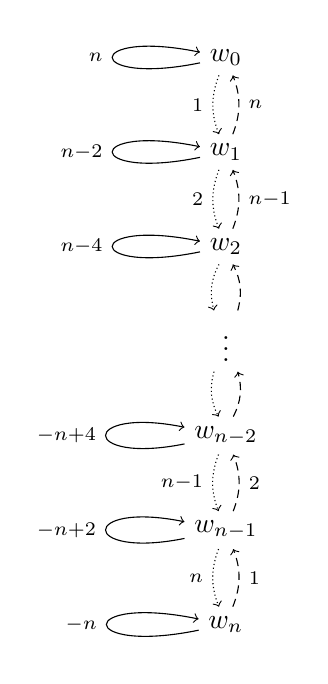
\begin{tikzpicture}[
              yscale = 1.2,
              bendy/.style = {bend right = 25},
              loopy/.style = {out = 190, in = 170, looseness = 40}
            ]
            % nodes
            \node (w0)   at (0,  0) {$w_0$};
            \node (w1)   at (0, -1) {$w_1$};
            \node (w2)   at (0, -2) {$w_2$};
            \node (rest) at (0, -3) {$\vdots$};
            \node (wn-2) at (0, -4) {$w_{n-2}$};
            \node (wn-1) at (0, -5) {$w_{n-1}$};
            \node (wn)   at (0, -6) {$w_n$};
            % the action of h
            \draw[->] (w0)    to[loopy] node[left]{$\scriptstyle n$} (w0);
            \draw[->] (w1)    to[loopy] node[left]{$\scriptstyle n-2$} (w1);
            \draw[->] (w2)    to[loopy] node[left]{$\scriptstyle n-4$} (w2);
            \draw[->] (wn-2)  to[loopy, looseness = 22.5] node[left]{$\scriptstyle -n+4$} (wn-2);
            \draw[->] (wn-1)  to[loopy, looseness = 22.5] node[left]{$\scriptstyle -n+2$} (wn-1);
            \draw[->] (wn)    to[loopy] node[left]{$\scriptstyle -n$} (wn);
            % the action of f
            \draw[->, densely dotted] (w0)    to[bendy] node[left] {$\scriptstyle 1$} (w1);
            \draw[->, densely dotted] (w1)    to[bendy] node[left] {$\scriptstyle 2$} (w2);
            \draw[->, densely dotted] (w2)    to[bendy] (rest);
            \draw[->, densely dotted] (rest)  to[bendy] (wn-2);
            \draw[->, densely dotted] (wn-2)  to[bendy] node[left] {$\scriptstyle n-1$} (wn-1);
            \draw[->, densely dotted] (wn-1)  to[bendy] node[left] {$\scriptstyle n$} (wn);
            % the action of e
            \draw[->, densely dashed] (w1)    to[bendy] node[right] {$\scriptstyle n$} (w0);
            \draw[->, densely dashed] (w2)    to[bendy] node[right] {$\scriptstyle n-1$} (w1);
            \draw[->, densely dashed] (rest)  to[bendy] (w2);
            \draw[->, densely dashed] (wn-2)  to[bendy] (rest);
            \draw[->, densely dashed] (wn-1)  to[bendy] node[right] {$\scriptstyle 2$} (wn-2);
            \draw[->, densely dashed] (wn)    to[bendy] node[right] {$\scriptstyle 1$} (wn-1);
          \end{tikzpicture}
        \end{center}
        \caption{%
          The irreducible representation~$\irred(n)$ of~$\Univ(\sllie_2)$.
          Loops depict the action of~$H$, dashed arrows the action of~$E$ and dotted arrows the action of~$F$.
        }
        \label{graphical representation of irreducible representation}
      \end{figure}
  \end{enumerate}
\end{theorem}

We refer to \cref{appendix representation theory of sl2} for more details on the representation theory of the Lie algebra~$\sllie_2$ in characteristic~zero.






\section{The Algebra~$\Univ_q(\sllie_2)$}

\begin{convention}
  In the following~$\kf$ denotes a field of characteristic zero and~$q$ is an element of~$\kf$ with~$q \neq 0, 1, -1$.
\end{convention}

\begin{definition}
  The~\algebra{$\kf$}~$\Univ_q(\sllie_2)$ is given by the generators
  \begin{gather}
    E \,,
    \quad
    K \,,
    \quad
    K^{-1} \,,
    \quad
    F
    \notag
  \shortintertext{subject to the relations}
    K K^{-1} = 1 = K^{-1} K \,,
    \quad
    K E = q^2 E K \,,
    \quad
    K F = q^{-2} F K \,,
    \quad
    E F - F E = \frac{K - K^{-1}}{q - q^{-1}} \,.
    \label{standard presentation}
  \end{gather}
\end{definition}

\begin{remark}[Choice of~$q$]
  One often requires additional conditions on~$q$, namely that
  \begin{enumerate}
    \item
      $q$ is not a root of unity, or that
    \item
      $\kf$ is the field~$\Kf(q)$ over some other field~$\Kf$, with~$q$ being the indeterminate.
  \end{enumerate}
\end{remark}

\begin{remark}[The case~$q = 1$]
  \label{quantum U1}
  The algebra~$\Univ_q(\sllie)$ admits another useful presentation:
  One introduces the element
  \[
    \widetilde{H}
    \defined
    \frac{K - K^{-1}}{q - q^{-1}}
  \]
  as an additional generator, and then adjust the relations~\eqref{standard presentation}.
  This presentation of~$\Univ_q(\sllie_2)$ does then make sense for any~$q \in \kf$, and for~$q = 1$ one has
  \[
    \Univ_1(\sllie_2)
    \cong
    \Univ(\sllie_2)[\sigma]/(\sigma^2 - 1)
  \]
  given by
  \begin{equation}
    \label{isomorphism for U1}
    E \mapsto \sigma E \,,
    \quad
    \widetilde{H} \mapsto \sigma H \,,
    \quad
    F \mapsto F \,,
    \quad
    K \mapsto \sigma \,.
  \end{equation}
  We refer to \cref{alternative presentation for quantum sl2} for more details on this presentation.
\end{remark}

\begin{remark}
  One might think about~$E$ and~$F$ as the usual elements of~$\sllie_2$, but~$\Univ_q(\sllie_2)$ does not contain the element~$H$.
  We will later see that the algebra~$\Univ_q(\sllie)$ lives (up to some technical details) inside an~\algebra{$\kfhbar$}~$\Univ_{\hbar}(\sllie_2)$ that also contains~$H$, and in which
  \[
    q = \e^{\hbar} \,,
    \quad
    K = \e^{\hbar H} \,.
  \]
  We may therefore think about the element~$K$ as
  \[
    K
    =
    q^H \,.
  \]
\end{remark}

\begin{theorem}[PBW basis]
  \label{quantum pbw}
  The algebra~$\Univ_q(\sllie_2)$ has a vector space basis given by
  \[
    F^l K^m E^n
    \qquad
    \text{with~$l, n \in \Natural$ and~$m \in \Integer$} 
  \]
\end{theorem}

\begin{proof}
  See \cref{proof of quantum pbw}.
\end{proof}

We refer to \cref{algebra structure of quantum sl2} for more remarks on the algebra structure of~$\Univ_q(\sllie_2)$.





\section{Representation Theory of~$\Univ_q(\sllie_2)$}

We will in this section focus on the finite-dimensional representation theory of~$\Univ_q(\sllie_2)$.



\subsection{The Case~$q = 1$}
\label{representation theory of quantum U1}

Every~\representation{$\sllie_2$} extends to a~\module{$\Univ_1(\sllie_1)$} by letting~$\sigma$ act by either~$1$ or~$-1$.
The resultings~\modules{$\Univ_1(\sllie_1)$} are denoted by~$\irred(\varepsilon, n)$ for~$\varepsilon = \pm$ and~$n \in \Natural$.
One can conclude from \cref{irreps of sl2} that every finite-dimensional~\module{$\Univ_1(\sllie_2)$} is semisimple, and that the irreducible finite-dimensional~\modules{$\Univ_1(\sllie_2)$} are given precisely given by~$\irred(\pm, n)$.
One can depict these irreducible modules as in \cref{graphical representation of quantum irreducible representation for q = 1}.
\begin{figure}
  \begin{center}
    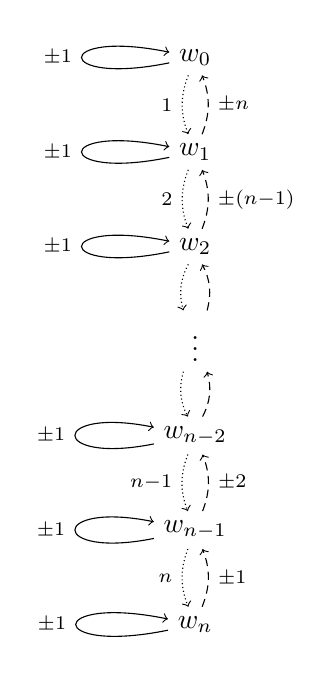
\begin{tikzpicture}[
        yscale = 1.2,
        bendy/.style = {bend right = 25},
        loopy/.style = {out = 190, in = 170, looseness = 40}
      ]
      % nodes
      \node (w0)   at (0,  0) {$w_0$};
      \node (w1)   at (0, -1) {$w_1$};
      \node (w2)   at (0, -2) {$w_2$};
      \node (rest) at (0, -3) {$\vdots$};
      \node (wn-2) at (0, -4) {$w_{n-2}$};
      \node (wn-1) at (0, -5) {$w_{n-1}$};
      \node (wn)   at (0, -6) {$w_n$};
      % the action of K
      \draw[->] (w0)    to[loopy] node[left]{$\scriptstyle \pm 1$} (w0);
      \draw[->] (w1)    to[loopy] node[left]{$\scriptstyle \pm 1$} (w1);
      \draw[->] (w2)    to[loopy] node[left]{$\scriptstyle \pm 1$} (w2);
      \draw[->] (wn-2)  to[loopy, looseness = 22.5] node[left]{$\scriptstyle \pm 1$} (wn-2);
      \draw[->] (wn-1)  to[loopy, looseness = 22.5] node[left]{$\scriptstyle \pm 1$} (wn-1);
      \draw[->] (wn)    to[loopy] node[left]{$\scriptstyle \pm 1$} (wn);
      % the action of F
      \draw[->, densely dotted] (w0)    to[bendy] node[left] {$\scriptstyle 1$} (w1);
      \draw[->, densely dotted] (w1)    to[bendy] node[left] {$\scriptstyle 2$} (w2);
      \draw[->, densely dotted] (w2)    to[bendy] (rest);
      \draw[->, densely dotted] (rest)  to[bendy] (wn-2);
      \draw[->, densely dotted] (wn-2)  to[bendy] node[left] {$\scriptstyle n-1$} (wn-1);
      \draw[->, densely dotted] (wn-1)  to[bendy] node[left] {$\scriptstyle n$} (wn);
      % the action of E
      \draw[->, densely dashed] (w1)    to[bendy] node[right] {$\scriptstyle \pm n$} (w0);
      \draw[->, densely dashed] (w2)    to[bendy] node[right] {$\scriptstyle \pm (n-1)$} (w1);
      \draw[->, densely dashed] (rest)  to[bendy] (w2);
      \draw[->, densely dashed] (wn-2)  to[bendy] (rest);
      \draw[->, densely dashed] (wn-1)  to[bendy] node[right] {$\scriptstyle \pm 2$} (wn-2);
      \draw[->, densely dashed] (wn)    to[bendy] node[right] {$\scriptstyle \pm 1$} (wn-1);
    \end{tikzpicture}
    \hspace{4em}
    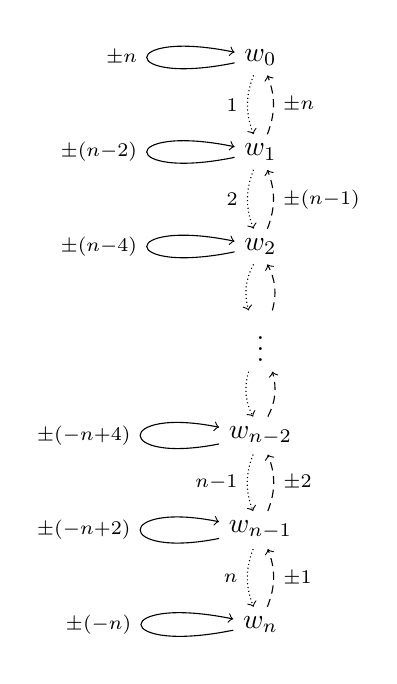
\begin{tikzpicture}[
        yscale = 1.2,
        bendy/.style = {bend right = 25},
        loopy/.style = {out = 190, in = 170, looseness = 40}
      ]
      % nodes
      \node (w0)   at (0,  0) {$w_0$};
      \node (w1)   at (0, -1) {$w_1$};
      \node (w2)   at (0, -2) {$w_2$};
      \node (rest) at (0, -3) {$\vdots$};
      \node (wn-2) at (0, -4) {$w_{n-2}$};
      \node (wn-1) at (0, -5) {$w_{n-1}$};
      \node (wn)   at (0, -6) {$w_n$};
      % the action of K
      \draw[->] (w0)    to[loopy] node[left]{$\scriptstyle \pm n$} (w0);
      \draw[->] (w1)    to[loopy] node[left]{$\scriptstyle \pm (n-2)$} (w1);
      \draw[->] (w2)    to[loopy] node[left]{$\scriptstyle \pm (n-4)$} (w2);
      \draw[->] (wn-2)  to[loopy, looseness = 22.5] node[left]{$\scriptstyle \pm (-n+4)$} (wn-2);
      \draw[->] (wn-1)  to[loopy, looseness = 22.5] node[left]{$\scriptstyle \pm (-n+2)$} (wn-1);
      \draw[->] (wn)    to[loopy] node[left]{$\scriptstyle \pm (-n)$} (wn);
      % the action of F
      \draw[->, densely dotted] (w0)    to[bendy] node[left] {$\scriptstyle 1$} (w1);
      \draw[->, densely dotted] (w1)    to[bendy] node[left] {$\scriptstyle 2$} (w2);
      \draw[->, densely dotted] (w2)    to[bendy] (rest);
      \draw[->, densely dotted] (rest)  to[bendy] (wn-2);
      \draw[->, densely dotted] (wn-2)  to[bendy] node[left] {$\scriptstyle n-1$} (wn-1);
      \draw[->, densely dotted] (wn-1)  to[bendy] node[left] {$\scriptstyle n$} (wn);
      % the action of E
      \draw[->, densely dashed] (w1)    to[bendy] node[right] {$\scriptstyle \pm n$} (w0);
      \draw[->, densely dashed] (w2)    to[bendy] node[right] {$\scriptstyle \pm (n-1)$} (w1);
      \draw[->, densely dashed] (rest)  to[bendy] (w2);
      \draw[->, densely dashed] (wn-2)  to[bendy] (rest);
      \draw[->, densely dashed] (wn-1)  to[bendy] node[right] {$\scriptstyle \pm 2$} (wn-2);
      \draw[->, densely dashed] (wn)    to[bendy] node[right] {$\scriptstyle \pm 1$} (wn-1);
    \end{tikzpicture}
  \end{center}
  \caption{%
    The irreducible representations~$\irred(\pm, n)$ of~$\Univ_1(\sllie_2)$.
    On the left side loops depict the action of~$K$, and on the right side they depict the action of~$\widetilde{H}$.
    On both sides dashed arrows depict the action of~$E$ and dotted arrows depict the action of~$F$.
  }
  \label{graphical representation of quantum irreducible representation for q = 1}
\end{figure}
We refer to \cref{representation theory of U1} for proofs of these claims.

We will keep the case of~$\Univ_1(\sllie_2)$ in the back of our minds while considering the following discussion.


\subsection{Weight Space Decomposition}

\begin{convention}
  In the following~$q$ is an element of~$\kf$ which is not a root of unity, unless otherwise specified.
\end{convention}

\begin{definition}
  Let~$M$ be an~\module{$\Univ_q(\sllie_2)$}.
  For every scalar~$\lambda \in \kf^{\times}$ the associated \defemph{weight space} is given by
  \[
    M_\lambda
    \defined
    \{
      m \in M
    \suchthat
      K m = \lambda m
    \} \,.
  \]
\end{definition}

\begin{theorem}
  \label{quantum weight decomposition}
  Let~$M$ be an~\module{$\Univ_q(\sllie_2)$}.
  \begin{enumerate}
    \item
      It holds for every scalar~$\lambda \in \kf^{\times}$ that
      \[
        E M_\lambda \subseteq M_{q^2 \lambda} \,,
        \quad
        F M_\lambda \subseteq M_{q^{-2} \lambda} \,.
      \]
    \item
      If~$M$ is finite-dimensional then~$M$ decomposes into weight spaces, and all occuring weights are of the form~$\pm q^n$ with~$n \in \Integer$.
  \end{enumerate}
\end{theorem}

\begin{proof}
  See \cref{proof of quantum weight decomposition}.
\end{proof}



\subsection{Verma Modules and Classifications}

\begin{definition}
  Let~$M$ be an~\module{$\Univ_q(\sllie_2)$}.
  \begin{enumerate}
    \item
      A weight vector~$m$ is \defemph{primitive} if it is nonzero and~$Em = 0$.
    \item
      The module~$M$ is of \defemph{highest weight~$\lambda$} if it is generated by a primitive weight vector of weight~$\lambda$.
  \end{enumerate}
\end{definition}

\begin{proposition}
  Every irreducible, finite-dimensional~\module{$\Univ_q(\sllie_2)$} is a highest weight module.
\end{proposition}

\begin{proof}
  The assertion follows from \cref{quantum weight decomposition}.
\end{proof}

We will classify the irreducible highest-weight representations of~$\Univ_q(\sllie_2)$ and its irreducible finite-dimensional representations.
We mirror the corresponding classifications of~\representations{$\sllie_2$}.

\begin{definition}
  Let~$\Univ_q(\blie)$ be the subalgebra of~$\Univ_q(\sllie_2)$ generated by~$E$,~$K$,~$K^{-1}$.%
  \footnote{
    Here~$\blie$ refers to the Lie subalgebra of~$\sllie_2$ consisting of the traceless upper triangular matrices, see \cref{appendix representation theory of sl2}.
  }
\end{definition}

\begin{definition}
  Let~$\lambda \in \kf^\times$.
  \begin{enumerate}
    \item
      Let~$\kf_\lambda$ be the one-dimensional~\module{$\Univ_q(\blie)$} whose underlying vector space is given by~$\kf$, together with the action
      \[
        K \cdot 1 = \lambda \,,
        \quad
        E \cdot 1 = 0 \,.
      \]
    \item
      The \defemph{Verma module} associated to~$\lambda$ is the~\module{$\Univ_q(\sllie_2)$} given by
      \[
        \verma(\lambda)
        \defined
        \Univ_q(\sllie_2) \tensor_{\Univ_q(\blie)} \kf_\lambda \,.
      \]
  \end{enumerate}
\end{definition}

\begin{definition}
  \label{definition of quantum integers}
  For~$q \in \kf$ with~$q \neq 0$ the \defemph{\howmanyth{$n$} quantum integer} is
  \[
    \qnum{n}
    \defined
    q^{n-1} + q^{n-3} + \dotsb + q^{-n+3} + q^{-n+1} \,,
  \]
  and thus for~$q \neq 1, 0, -1$,
  \[
    \qnum{n}
    =
    \frac{q^n - q^{-n}}{q - q^{-1}} \,.
  \]
  The \defemph{quantum factorial} is
  \[
    \qnum{n}!
    \defined
    \qnum{n} \qnum{n-1} \dotsm \qnum{1} \,.
  \]
  For every invertible element~$x \in \Univ_q(\sllie_2)$ and integer~$n \in \Integer$ let
  \[
    \qnum{x, n}
    \defined
    \frac{ q^n x - q^{-n} x^{-1} }{ q - q^{-1} } \,.
  \]
\end{definition}

\begin{remark}
  For~$q = 1$ we have~$\qnum{n}[1] = n$ and~$\qnum{n}[1]! = n!$.
\end{remark}

\begin{proposition}
  \label{understanding quantum verma modules}
  Let~$\lambda \in \kf^\times$.
  \begin{enumerate}
    \item
      The Verma module~$\verma(\lambda)$ has the basis
      \[
        m_i
        \defined
        F^i \tensor 1
        \qquad
        \text{with~$i \geq 0$,}
      \]
      and the actions of~$E$,~$K$,~$F$ on this basis is given by
      \[
        F m_i = m_{i+1} \,,
        \quad
        K m_i = q^{-2i} \lambda m_i \,,
        \quad
        E m_i = \qnum{i} \qnum{\lambda, 1-i} m_{i-1} \,.
      \]
      This action can be graphically described as in \cref{graphical representation of quantum verma module}.
      \begin{figure}
        \begin{center}
          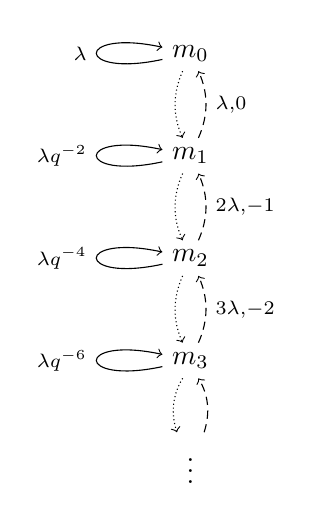
\begin{tikzpicture}[
              yscale = 1.3,
              bendy/.style = {bend right = 30},
              loopy/.style = {out = 190, in = 170, looseness = 30}
            ]
            % nodes
            \node (m0)   at (0,  0) {$m_0$};
            \node (m1)   at (0, -1) {$m_1$};
            \node (m2)   at (0, -2) {$m_2$};
            \node (m3)   at (0, -3) {$m_3$};
            \node (rest) at (0, -4) {$\vdots$};
            % the action of f
            \draw[->, densely dotted] (m0) to[bendy] (m1);
            \draw[->, densely dotted] (m1) to[bendy] (m2);
            \draw[->, densely dotted] (m2) to[bendy] (m3);
            \draw[->, densely dotted] (m3) to[bendy] (rest);
            % the action of e
            \draw[->, densely dashed] (m1)   to[bendy] node[right] {$\scriptstyle \qnum{\lambda, 0}$} (m0);
            \draw[->, densely dashed] (m2)   to[bendy] node[right] {$\scriptstyle \qnum{2} \qnum{\lambda, -1}$} (m1);
            \draw[->, densely dashed] (m3)   to[bendy] node[right] {$\scriptstyle \qnum{3} \qnum{\lambda, -2}$} (m2);
            \draw[->, densely dashed] (rest) to[bendy] (m3);
            % the action of h
            \draw[->] (m0) to[loopy] node[left]{$\scriptstyle \lambda$} (m0);
            \draw[->] (m1) to[loopy] node[left]{$\scriptstyle \lambda q^{-2}$} (m1);
            \draw[->] (m2) to[loopy] node[left]{$\scriptstyle \lambda q^{-4}$} (m2);
            \draw[->] (m3) to[loopy] node[left]{$\scriptstyle \lambda q^{-6}$} (m3);
          \end{tikzpicture}
          \hspace{4em}
          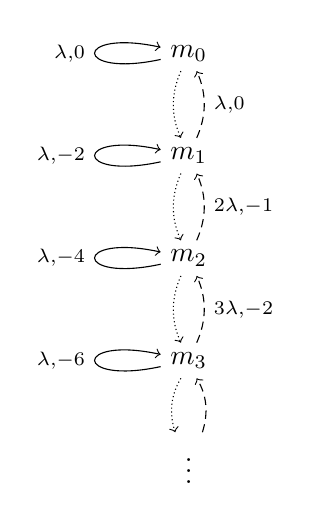
\begin{tikzpicture}[
              yscale = 1.3,
              bendy/.style = {bend right = 30},
              loopy/.style = {out = 190, in = 170, looseness = 30}
            ]
            % nodes
            \node (m0)   at (0,  0) {$m_0$};
            \node (m1)   at (0, -1) {$m_1$};
            \node (m2)   at (0, -2) {$m_2$};
            \node (m3)   at (0, -3) {$m_3$};
            \node (rest) at (0, -4) {$\vdots$};
            % the action of f
            \draw[->, densely dotted] (m0) to[bendy] (m1);
            \draw[->, densely dotted] (m1) to[bendy] (m2);
            \draw[->, densely dotted] (m2) to[bendy] (m3);
            \draw[->, densely dotted] (m3) to[bendy] (rest);
            % the action of e
            \draw[->, densely dashed] (m1)   to[bendy] node[right] {$\scriptstyle \qnum{\lambda, 0}$} (m0);
            \draw[->, densely dashed] (m2)   to[bendy] node[right] {$\scriptstyle \qnum{2} \qnum{\lambda, -1}$} (m1);
            \draw[->, densely dashed] (m3)   to[bendy] node[right] {$\scriptstyle \qnum{3} \qnum{\lambda, -2}$} (m2);
            \draw[->, densely dashed] (rest) to[bendy] (m3);
            % the action of h
            \draw[->] (m0) to[loopy] node[left]{$\scriptstyle \qnum{\lambda,  0}$} (m0);
            \draw[->] (m1) to[loopy] node[left]{$\scriptstyle \qnum{\lambda, -2}$} (m1);
            \draw[->] (m2) to[loopy] node[left]{$\scriptstyle \qnum{\lambda, -4}$} (m2);
            \draw[->] (m3) to[loopy] node[left]{$\scriptstyle \qnum{\lambda, -6}$} (m3);
          \end{tikzpicture}
        \end{center}
        \caption{
          The Verma module~$\verma(\lambda)$ of~$\Univ_q(\sllie_2)$.
          On the left side loops depict the action of~$K$, an on the right side they depict the action of~$\widetilde{H}$.
          On both sides the action of~$F$ is depicted by dotted arrows and the action of~$E$ by dashed arrows.
        }
        \label{graphical representation of quantum verma module}
      \end{figure}
    \item
      The Verma module~$\verma(\lambda)$ is indecomposable.
    \item
      \begin{enumerate}
        \item
          If~$\lambda = \pm q^n$ for some~$n \in \Natural$ then the Verma module~$\verma(\lambda)$ contains a unique nonzero, proper submodule~$N_\lambda$, which is spanned by the elements
          \[
            m_i
            \qquad
            \text{with~$i \geq n+1$.}
          \]
          This submodule is isomorphic to~$\verma(q^{-n-2} \lambda)$.
        \item
          If~$\lambda \neq \pm q^n$ for every~$n \in \Natural$ then the Verma module~$\verma(\lambda)$ is irreducible.
      \end{enumerate}
  \end{enumerate}
\end{proposition}

\begin{proof}
  See \cref{proof of understanding quantum verma modules}.
\end{proof}

\begin{definition}
  For every scalar~$\lambda \in \kf^\times$ let
  \[
    \irred(\lambda)
    \defined
    \begin{cases*}
        \verma(\lambda) / N_\lambda
        &
        if~$\lambda = \pm q^n$ for some~$n \in \Natural$,
        \\
        \verma(\lambda)
        &
        otherwise.
    \end{cases*}
  \]
\end{definition}

\begin{theorem}
  \leavevmode
  \begin{enumerate}
    \item
      There is a one-to-one correspondence given by
      \begin{align*}
        \kf^\times
        &\longmapsto
        \left\{
          \begin{tabular}{@{}c@{}}
            isomorphism clases of \\
            highest-weight irreducible \\
            \modules{$\Univ_q(\sllie_2)$}
          \end{tabular}
        \right\} \,,
        \\
        \lambda
        &\longmapsto
        \irred(\lambda) \,.
      \end{align*}
    \item
      The module~$\irred(\lambda)$ is finite-dimensional if and only if~$\lambda = \pm q^n$ for some~$n \in \Natural$.
      The above one-to-one correspondence does therefore restrict to a one-to-one correspondence given by
      \begin{align*}
        \{ 1, -1 \} \times \Natural
        &\longmapsto
        \left\{
          \begin{tabular}{@{}c@{}}
            isomorphism clases of \\
            finite-dimensional irreducible \\
            \modules{$\Univ_q(\sllie_2)$}
          \end{tabular}
        \right\} \,,
        \\
        (\varepsilon, n)
        &\longmapsto
        \irred(\varepsilon q^n) \,.
      \end{align*}
      We have for every~$n \in \Natural$ that
      \[
        \dim(\irred(\pm q^n))
        =
        n + 1 \,.
      \]
  \end{enumerate}
\end{theorem}


% TODO: Add a proof in the appendix.


\begin{remark}
  \leavevmode
  \begin{enumerate}
    \item
      For every~$n \in \Integer$ we have
      \[
        \qnum{\pm q^n, -i+1}
        =
        \pm \qnum{n-i+1} \,.
      \]
      On the rescalled basis~$m_0, \dotsc, m_n$ of~$\irred(\pm q^n)$ given by
      \[
        w_i
        \defined
        \frac{m_i}{\qnum{i}!}
      \]
      the actions of~$E$,~$K$,~$F$ thus become
      \[
        E w_i = \pm \qnum{n-i+1} w_{i-1} \,,
        \quad
        K w_i = \pm q^{n-2i} w_i \,,
        \quad
        F w_i = \qnum{i+1} w_{i+1} \,.
      \]
      The action of~$E$,~$K$,~$F$ on~$\irred(\pm q^n)$ can therefore be graphically be represented as in \cref{graphical representation of irreducible quantum representation}.
      \begin{figure}[t]
        \begin{center}
          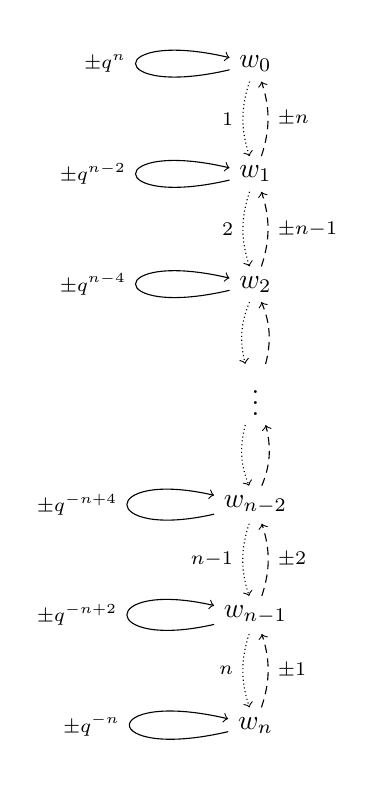
\begin{tikzpicture}[
              yscale = 1.4,
              bendy/.style = {bend right = 25},
              loopy/.style = {out = 190, in = 170, looseness = 50}
            ]
            % nodes
            \node (w0)   at (0,  0) {$w_0$};
            \node (w1)   at (0, -1) {$w_1$};
            \node (w2)   at (0, -2) {$w_2$};
            \node (rest) at (0, -3) {$\vdots$};
            \node (wn-2) at (0, -4) {$w_{n-2}$};
            \node (wn-1) at (0, -5) {$w_{n-1}$};
            \node (wn)   at (0, -6) {$w_n$};
            % the action of h
            \draw[->] (w0)    to[loopy] node[left]{$\scriptstyle \pm q^n$} (w0);
            \draw[->] (w1)    to[loopy] node[left]{$\scriptstyle \pm q^{n-2}$} (w1);
            \draw[->] (w2)    to[loopy] node[left]{$\scriptstyle \pm q^{n-4}$} (w2);
            \draw[->] (wn-2)  to[loopy, looseness = 29] node[left]{$\scriptstyle \pm q^{-n+4}$} (wn-2);
            \draw[->] (wn-1)  to[loopy, looseness = 29] node[left]{$\scriptstyle \pm q^{-n+2}$} (wn-1);
            \draw[->] (wn)    to[loopy] node[left]{$\scriptstyle \pm q^{-n}$} (wn);
            % the action of f
            \draw[->, densely dotted] (w0)    to[bendy] node[left] {$\scriptstyle \qnum{1}$} (w1);
            \draw[->, densely dotted] (w1)    to[bendy] node[left] {$\scriptstyle \qnum{2}$} (w2);
            \draw[->, densely dotted] (w2)    to[bendy] (rest);
            \draw[->, densely dotted] (rest)  to[bendy] (wn-2);
            \draw[->, densely dotted] (wn-2)  to[bendy] node[left] {$\scriptstyle \qnum{n-1}$} (wn-1);
            \draw[->, densely dotted] (wn-1)  to[bendy] node[left] {$\scriptstyle \qnum{n}$} (wn);
            % the action of e
            \draw[->, densely dashed] (w1)    to[bendy] node[right] {$\scriptstyle \pm \qnum{n}$} (w0);
            \draw[->, densely dashed] (w2)    to[bendy] node[right] {$\scriptstyle \pm \qnum{n-1}$} (w1);
            \draw[->, densely dashed] (rest)  to[bendy] (w2);
            \draw[->, densely dashed] (wn-2)  to[bendy] (rest);
            \draw[->, densely dashed] (wn-1)  to[bendy] node[right] {$\scriptstyle \pm \qnum{2}$} (wn-2);
            \draw[->, densely dashed] (wn)    to[bendy] node[right] {$\scriptstyle \pm \qnum{1}$} (wn-1);
          \end{tikzpicture}
          \hspace{4em}
          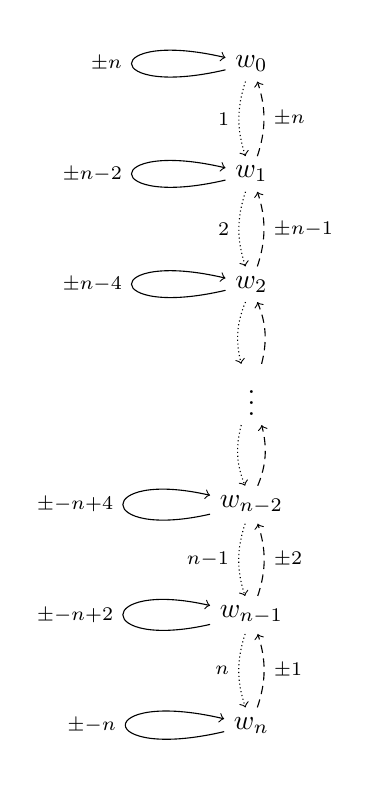
\begin{tikzpicture}[
              yscale = 1.4,
              bendy/.style = {bend right = 25},
              loopy/.style = {out = 190, in = 170, looseness = 50}
            ]
            % nodes
            \node (w0)   at (0,  0) {$w_0$};
            \node (w1)   at (0, -1) {$w_1$};
            \node (w2)   at (0, -2) {$w_2$};
            \node (rest) at (0, -3) {$\vdots$};
            \node (wn-2) at (0, -4) {$w_{n-2}$};
            \node (wn-1) at (0, -5) {$w_{n-1}$};
            \node (wn)   at (0, -6) {$w_n$};
            % the action of h
            \draw[->] (w0)    to[loopy] node[left]{$\scriptstyle \pm \qnum{n}$} (w0);
          \draw[->] (w1)    to[loopy] node[left]{$\scriptstyle \pm \qnum{n-2}$} (w1);
            \draw[->] (w2)    to[loopy] node[left]{$\scriptstyle \pm \qnum{n-4}$} (w2);
            \draw[->] (wn-2)  to[loopy, looseness = 29] node[left]{$\scriptstyle \pm \qnum{-n+4}$} (wn-2);
            \draw[->] (wn-1)  to[loopy, looseness = 29] node[left]{$\scriptstyle \pm \qnum{-n+2}$} (wn-1);
            \draw[->] (wn)    to[loopy] node[left]{$\scriptstyle \pm \qnum{-n}$} (wn);
            % the action of f
            \draw[->, densely dotted] (w0)    to[bendy] node[left] {$\scriptstyle \qnum{1}$} (w1);
            \draw[->, densely dotted] (w1)    to[bendy] node[left] {$\scriptstyle \qnum{2}$} (w2);
            \draw[->, densely dotted] (w2)    to[bendy] (rest);
            \draw[->, densely dotted] (rest)  to[bendy] (wn-2);
            \draw[->, densely dotted] (wn-2)  to[bendy] node[left] {$\scriptstyle \qnum{n-1}$} (wn-1);
            \draw[->, densely dotted] (wn-1)  to[bendy] node[left] {$\scriptstyle \qnum{n}$} (wn);
            % the action of e
            \draw[->, densely dashed] (w1)    to[bendy] node[right] {$\scriptstyle \pm \qnum{n}$} (w0);
            \draw[->, densely dashed] (w2)    to[bendy] node[right] {$\scriptstyle \pm \qnum{n-1}$} (w1);
            \draw[->, densely dashed] (rest)  to[bendy] (w2);
            \draw[->, densely dashed] (wn-2)  to[bendy] (rest);
            \draw[->, densely dashed] (wn-1)  to[bendy] node[right] {$\scriptstyle \pm \qnum{2}$} (wn-2);
            \draw[->, densely dashed] (wn)    to[bendy] node[right] {$\scriptstyle \pm \qnum{1}$} (wn-1);
          \end{tikzpicture}
        \end{center}
        \caption{
          The irreducible representations~$\irred(\pm q^n)$ of~$\Univ_q(\sllie_2)$.
          On the left side the loops depict the action of~$K$, an on the right side they depict the action of~$\widetilde{H}$.
          On both sides the action of~$F$ is depicted by dotted arrows and the action of~$E$ by dashed arrows.
        }
        \label{graphical representation of irreducible quantum representation}
      \end{figure}
    \item
      We can consider again the element
      \[
        \widetilde{H}
        \defined
        \frac{K - K^{-1}}{q - q^{-1}}
      \]
      of~$\Univ_q(\sllie_2)$.
      It acts on the weight space~$M_{\lambda q^{-2i}}$ by the scalar~$\qnum{\lambda, -2i}$.
      For~$\lambda = \pm q^n$ this means
      \[
        \qnum{\lambda, -2i}
        =
        \qnum{\pm q^n, -2i}
        =
        \pm \qnum{n - 2i} \,.
      \]
      The action of~$\widetilde{H}$ on the Verma module~$\verma(\lambda)$ and irreducible modules~$\irred(\pm q^n)$ is therefore as depicted in \cref{graphical representation of quantum verma module} and \cref{graphical representation of irreducible quantum representation}.
    \item
      We observe that for~$q = 1$ the descriptions of the irreducible~\modules{$\Univ_q(\sllie_2)$}~$\irred(\pm q^n)$ from \cref{graphical representation of irreducible quantum representation} becomes the description of the irreducible~\modules{$\Univ_1(\sllie_2)$}~$\irred(\pm, n)$ from~\cref{graphical representation of quantum irreducible representation for q = 1}.
  \end{enumerate}
\end{remark}



\subsection{Semisimplicity of Finite-Dimensional~$\Univ_q(\sllie_2)$-modules}

\begin{theorem}
  \label{finite-dimensional quantum modules are semisimple}
  Every finite-dimensional~\module{$\Univ_q(\sllie_2)$} is semisimple.
\end{theorem}

\begin{proof}[Proof]
  See \cref{proof of finite-dimensional quantum modules are semisimple}.
\end{proof}
  
\begin{corollary}
  \label{decomposition from quantum weight spaces}
  Let~$M$,~$N$ be two finite-dimensional~\modules{$\Univ_q(\sllie_2)$} with~$\dim M_\lambda = \dim N_\lambda$ for every~$\lambda \in \kf^\times$.
  Then~$M \cong N$.
  \qed
\end{corollary}





\section{Hopf Algebra Structure on~$\Univ_q(\sllie_2)$}


\begin{proposition}
  \label{hopf algebra structure on quantum sl2}
  The algebra~$\Univ_q(\sllie_2)$ becomes a Hopf algebra when endowed with the comultiplication~$\Delta$, the counit~$\varepsilon$ and the antipode~$S$ given by
  \begin{gather*}
    \Delta(E) = E \tensor K + 1 \tensor E \,,
    \quad
    \Delta(F) = F \tensor 1 + K^{-1} \tensor F \,,
    \quad
    \Delta(K) = K \tensor K \,,
    \\
    \varepsilon(E) = 0 \,,
    \quad
    \varepsilon(F) = 0 \,,
    \quad
    \varepsilon(K) = 1
    \\
    S(E) = -E K^{-1} \,,
    \quad
    S(F) = -KF \,,
    \quad
    S(K) = K^{-1} \,.
  \end{gather*}
\end{proposition}

\begin{proof}
  One checks that the proposed images of the algebra generators~$E$,~$F$,~$K$,~$K^{-1}$ are compatible with the defining relations of~$\Univ_q(\sllie_2)$, and that the Hopf algebra diagram commute on these algebra generators.
\end{proof}

\begin{definition}
  The Hopf algebra structure of~$\Univ_q(\sllie_2)$ is given as in \cref{hopf algebra structure on quantum sl2}.
\end{definition}

\begin{remark}
%  \leavevmode
%  \begin{enumerate}
%    \item
      The Hopf algebra~$\Univ_q(\sllie_2)$ is neither commutative nor cocommutative.
      It is an example of a so-called \defemph{quantum group}.
%    \item
%      In~$\Univ_q(\sllie_2)$ we don’t have~$S^2 = \id$ but instead
%      \[
%        S^2(x) = K^{-1} x K
%      \]
%      for every element~$x \in \Univ_q(\sllie_2)$, as can be checked on the elements~$E$,~$K$,~$F$.
%      It entails in particular that
%      \[
%        S^2(E)
%        =
%        K^{-1} E K
%        =
%        q^2 K^{-1} K E
%        =
%        q^2 E \,,
%      \]
%      which shows that~$S$ has infinite order.
%  \end{enumerate}
\end{remark}

\begin{lemma}
  \label{quantum weight spaces of tensor product}
  Let~$M$,~$N$ be two finite-dimensional~\modules{$\Univ_q(\sllie_2)$}.
  Then
  \[
    (M \tensor N)_\lambda
    =
    \bigoplus_{\mu \kappa = \lambda}
    M_\mu \tensor N_\kappa \,.
  \]
\end{lemma}

\begin{proof}
  See \cref{proof of quantum weight spaces of tensor product}.
\end{proof}

\begin{corollary}
  Let~$M$,~$N$ be two finite-dimensional~\modules{$\Univ_q(\sllie_2)$}.
  Then
  \[
    M \tensor N
    \cong
    N \tensor M \,.
  \]
\end{corollary}

\begin{proof}
  This follows from \cref{decomposition from quantum weight spaces} and \cref{quantum weight spaces of tensor product}.
\end{proof}

\begin{warning}
  For two (finite-dimensional)~\modules{$\Univ_q(\sllie_2)$}~$M$,~$N$ the flip map
  \[
    \tau
    \colon
    M \tensor N
    \to
    N \tensor M \,,
    \quad
    m \tensor n
    \mapsto
    n \tensor m
  \]
  is in general not~\linear{$\Univ_q(\sllie_2)$}.
\end{warning}

\begin{example}
  Indeed, let us consider~$M = N = \irred(q)$ with basis~$m_0$,~$m_1$.
  Then
  \[
    F \cdot (m_0 \tensor m_1)
    =
    m_1 \tensor m_1
    \neq
    q m_1 \tensor m_1
    =
    F \cdot (m_1 \tensor m_0) \,.
  \]
\end{example}

There exists a quantum version of the Clebsch--Gordan formula, see \cref{quantum clebsch gordan}.



\section{Outlook: The Deformation~$\Univ_{\hbar}(\sllie_2)$}

\begin{definition}
  Let~$A$ be a Hopf algebra over~$\kf$.
  A \defemph{(formal) deformation} of a Hopf algebra~$A$ is a Hopf algebra over~$\kfhbar$ such that~$A_\hbar = \power{A}{\hbar}$ as~\modules{$\kfhbar$} and~$A_\hbar / \hbar A_\hbar = A$ as Hopf algebras over~$\kf$.
\end{definition}

\begin{remark}
%  Let~$A$ be a Hopf algebra over~$\kf$.
%  \begin{enumerate}
%    \item
      The above definition is actually wrong.
      Instead of simply Hopf algebras over~$\kfhbar$ one needs to consider \defemph{topological Hopf algebras}.
      This means that for the comultiplication of~$A_\hbar$ one has to replace the tensor product
      \[
        A_\hbar \tensor_{\kfhbar} A_\hbar
      \]
      by its~\adic{$\hbar$} completion
      \[
        A_\hbar \ctensor A_\hbar \,.
      \]
      In the given situation we have
      \[
        A_\hbar \ctensor A_\hbar
        =
        \power{A}{\hbar} \ctensor \power{A}{\hbar}
        \cong
        \power{(A \tensor A)}{\hbar}
      \]
      as~\modules{$\kfhbar$}.
      This means that we must allow the comultiplication to take as values not only tensors, but actually power series of tensors.
%    \item
%      If~$A_{\hbar}$ is a deformation of~$A$ then the multiplication
%      \[
%        m_{\hbar}
%        \colon
%        A_\hbar \times A_\hbar
%        \to
%        A_\hbar
%      \]
%      and the comultiplication
%      \[
%        \Delta_{\hbar}
%        \colon
%        A
%        \to
%        A_\hbar \ctensor A_\hbar
%      \]
%      are uniquely determined by the values
%      \[
%        \mu_{\hbar}(a,b) \,,
%        \quad
%        \Delta_{\hbar}(a)
%        \qquad
%        \text{with~$a, b \in A$.}
%      \]
%      These values are of the form
%      \begin{align*}
%        \mu_{\hbar}(a,b)
%        &=
%        \mu_0(a,b) + \mu_1(a,b) \hbar + \mu_2(a,b) \hbar^2 + \dotsb \,,
%        \\
%        \Delta_{\hbar}(a)
%        &=
%        \Delta_0(a) + \Delta_1(a) \hbar + \Delta_2(a) \hbar^2 + \dotsb
%      \end{align*}
%      for certain (bi)linear map
%      \[
%        \mu_i \colon A \times A \to A \,,
%        \quad
%        \Delta_i \colon A \to A \tensor A \,.
%      \]
%      It follows from the identity of Hopf algebras~$A_\hbar / \hbar A_\hbar = A$ that~$\mu_0$ needs to be the multiplication of~$A$ and~$\Delta_0$ the comultiplication of~$A$.
%      The Hopf algebra structure of~$A_\hbar$, is in this sense, a \enquote{perturbation} of the one of~$A$.
%  \end{enumerate}
\end{remark}

\begin{theorem}
  The universal enveloping algebra~$\Univ(\sllie_2)$ admits a Hopf algebra deformation
  \[
    \Univ_{\hbar}(\sllie_2)
  \]
  that is given by
  \begin{gather*}
    [H, E] = 2E \,,
    \quad
    [H, F] = -2F \,,
    \quad
    [E, F]
    =
    \frac{ \e^{\hbar H} - \e^{-\hbar H} }{ \e^{\hbar} - \e^{-\hbar} } \,,
    \\
    \Delta(E) = E \tensor \e^{\hbar H} + 1 \tensor E \,,
    \quad
    \Delta(H) = H \tensor 1 + 1 \tensor H \,,
    \quad
    \Delta(F) = F \tensor 1 + \e^{-\hbar H} \tensor F \,,
    \\
    \varepsilon(E) = 0 \,,
    \quad
    \varepsilon(H) = 0 \,,
    \quad
    \varepsilon(F) = 0 \,,
    \\
    S(E) = -E \e^{-\hbar H} \,,
    \quad
    S(H) = -H \,,
    \quad
    S(F) = - \e^{\hbar H} F \,.
  \end{gather*}
\end{theorem}

\begin{remark}
  \leavevmode
  \begin{enumerate}
    \item
      In the algebra~$\Univ_{\hbar}(\sllie_2)$ we can consider the well-defined elements
      \[
        q \defined \e^{\hbar} \,,
        \quad
        K \defined \e^{\hbar H} \,.
      \]
      The elements~$q$,~$E$,~$K$,~$K^{-1}$,~$F$ satisfy the defining relations of~$\Univ_q(\sllie_2)$.
      We can thus (up to some technical details) regard~$\Univ_q(\sllie_2)$ as a subalgebra of~$\Univ_{\hbar}(\sllie_2)$.
    \item
      In~$\Univ_{\hbar}(\sllie_2)$ we have both the element~$H$ and the element
      \[
        \widetilde{H}
        \defined
        [E,F]
        =
        \frac{K - K^{-1}}{q - q^{-1}}
        =
        \frac{\e^{\hbar H} - \e^{-\hbar H}}{\e^{\hbar} - \e^{-\hbar}}
      \]
      which is of the form
      \[
        \widetilde{H}
        =
        H + \text{terms of order~$\hbar^2$} \,.
      \]
      We may think about~$\widetilde{H}$ is a deformation of~$H$ (in an informal sense).
      We note that
      \[
        q \equiv 1 \,,
        \quad
        K \equiv 1 \,,
        \quad
        \widetilde{H} \equiv H
        \qquad
        \pMod{\hbar}.
      \]
  \end{enumerate}
\end{remark}

\begin{theorem}[{\cite[Proposition~6.4.10]{guide_to_quantum_groups}}]
  For every natural number~$n \in \Natural$ let~$L(n)$ be the free~\module{$\kfhbar$} of rank~$n+1$ with basis~$w_0, \dotsc, w_n$.
  \begin{enumerate}
    \item
      There exists a unique~\module{$\Univ_{\hbar}(\sllie_2)$} structure on~$V(n)$ such that
      \[
        H w_i \defined (n - 2i) w_i \,,
        \quad
        E w_i \defined \qnum{n - i + 1} w_{i-1} \,,
        \quad
        F w_i \defined \qnum{i+1} w_{i+1} \,.
      \]
      The actions of~$E$,~$H$,~$F$ can be graphically depicted as in \cref{graphical representation of deformed representations}. 
      \begin{figure}
        \begin{center}
          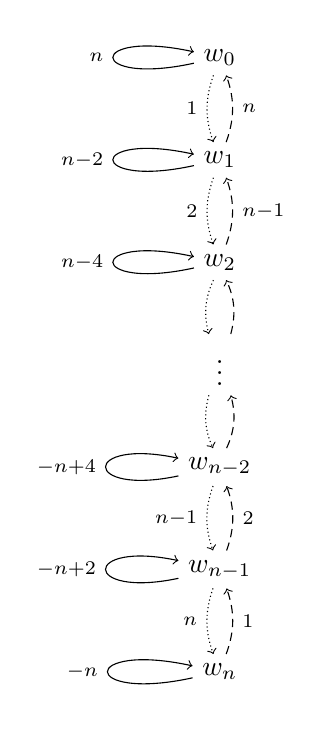
\begin{tikzpicture}[
              yscale = 1.3,
              bendy/.style = {bend right = 25},
              loopy/.style = {out = 190, in = 170, looseness = 40}
            ]
            % nodes
            \node (w0)   at (0,  0) {$w_0$};
            \node (w1)   at (0, -1) {$w_1$};
            \node (w2)   at (0, -2) {$w_2$};
            \node (rest) at (0, -3) {$\vdots$};
            \node (wn-2) at (0, -4) {$w_{n-2}$};
            \node (wn-1) at (0, -5) {$w_{n-1}$};
            \node (wn)   at (0, -6) {$w_n$};
            % the action of H
            \draw[->] (w0)    to[loopy] node[left]{$\scriptstyle n$} (w0);
            \draw[->] (w1)    to[loopy] node[left]{$\scriptstyle n-2$} (w1);
            \draw[->] (w2)    to[loopy] node[left]{$\scriptstyle n-4$} (w2);
            \draw[->] (wn-2)  to[loopy, looseness = 22.5] node[left]{$\scriptstyle -n+4$} (wn-2);
            \draw[->] (wn-1)  to[loopy, looseness = 22.5] node[left]{$\scriptstyle -n+2$} (wn-1);
            \draw[->] (wn)    to[loopy] node[left]{$\scriptstyle -n$} (wn);
            % the action of F
            \draw[->, densely dotted] (w0)    to[bendy] node[left] {$\scriptstyle \qnum{1}$} (w1);
            \draw[->, densely dotted] (w1)    to[bendy] node[left] {$\scriptstyle \qnum{2}$} (w2);
            \draw[->, densely dotted] (w2)    to[bendy] (rest);
            \draw[->, densely dotted] (rest)  to[bendy] (wn-2);
            \draw[->, densely dotted] (wn-2)  to[bendy] node[left] {$\scriptstyle \qnum{n-1}$} (wn-1);
            \draw[->, densely dotted] (wn-1)  to[bendy] node[left] {$\scriptstyle \qnum{n}$} (wn);
            % the action of E
            \draw[->, densely dashed] (w1)    to[bendy] node[right] {$\scriptstyle \qnum{n}$} (w0);
            \draw[->, densely dashed] (w2)    to[bendy] node[right] {$\scriptstyle \qnum{n-1}$} (w1);
            \draw[->, densely dashed] (rest)  to[bendy] (w2);
            \draw[->, densely dashed] (wn-2)  to[bendy] (rest);
            \draw[->, densely dashed] (wn-1)  to[bendy] node[right] {$\scriptstyle \qnum{2}$} (wn-2);
            \draw[->, densely dashed] (wn)    to[bendy] node[right] {$\scriptstyle \qnum{1}$} (wn-1);
          \end{tikzpicture}
          \hspace{3em}
          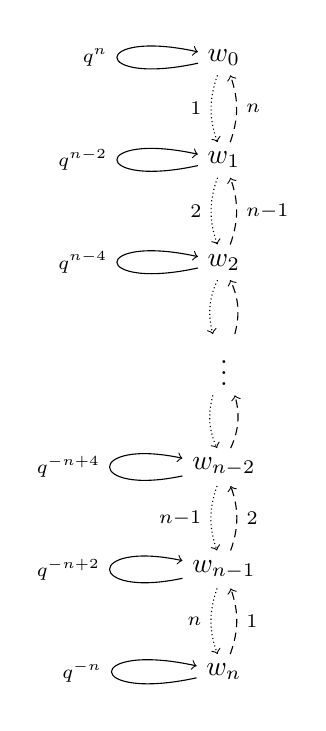
\begin{tikzpicture}[
              yscale = 1.3,
              bendy/.style = {bend right = 25},
              loopy/.style = {out = 190, in = 170, looseness = 40}
            ]
            % nodes
            \node (w0)   at (0,  0) {$w_0$};
            \node (w1)   at (0, -1) {$w_1$};
            \node (w2)   at (0, -2) {$w_2$};
            \node (rest) at (0, -3) {$\vdots$};
            \node (wn-2) at (0, -4) {$w_{n-2}$};
            \node (wn-1) at (0, -5) {$w_{n-1}$};
            \node (wn)   at (0, -6) {$w_n$};
            % the action of K
            \draw[->] (w0)    to[loopy] node[left]{$\scriptstyle q^n$} (w0);
            \draw[->] (w1)    to[loopy] node[left]{$\scriptstyle q^{n-2}$} (w1);
            \draw[->] (w2)    to[loopy] node[left]{$\scriptstyle q^{n-4}$} (w2);
            \draw[->] (wn-2)  to[loopy, looseness = 22.5] node[left]{$\scriptstyle q^{-n+4}$} (wn-2);
            \draw[->] (wn-1)  to[loopy, looseness = 22.5] node[left]{$\scriptstyle q^{-n+2}$} (wn-1);
            \draw[->] (wn)    to[loopy] node[left]{$\scriptstyle q^{-n}$} (wn);
            % the action of F
            \draw[->, densely dotted] (w0)    to[bendy] node[left] {$\scriptstyle \qnum{1}$} (w1);
            \draw[->, densely dotted] (w1)    to[bendy] node[left] {$\scriptstyle \qnum{2}$} (w2);
            \draw[->, densely dotted] (w2)    to[bendy] (rest);
            \draw[->, densely dotted] (rest)  to[bendy] (wn-2);
            \draw[->, densely dotted] (wn-2)  to[bendy] node[left] {$\scriptstyle \qnum{n-1}$} (wn-1);
            \draw[->, densely dotted] (wn-1)  to[bendy] node[left] {$\scriptstyle \qnum{n}$} (wn);
            % the action of E
            \draw[->, densely dashed] (w1)    to[bendy] node[right] {$\scriptstyle \qnum{n}$} (w0);
            \draw[->, densely dashed] (w2)    to[bendy] node[right] {$\scriptstyle \qnum{n-1}$} (w1);
            \draw[->, densely dashed] (rest)  to[bendy] (w2);
            \draw[->, densely dashed] (wn-2)  to[bendy] (rest);
            \draw[->, densely dashed] (wn-1)  to[bendy] node[right] {$\scriptstyle \qnum{2}$} (wn-2);
            \draw[->, densely dashed] (wn)    to[bendy] node[right] {$\scriptstyle \qnum{1}$} (wn-1);
          \end{tikzpicture}
          \hspace{3em}
          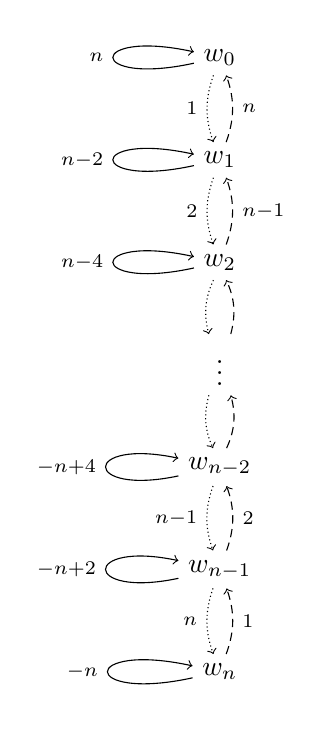
\begin{tikzpicture}[
              yscale = 1.3,
              bendy/.style = {bend right = 25},
              loopy/.style = {out = 190, in = 170, looseness = 40}
            ]
            % nodes
            \node (w0)   at (0,  0) {$w_0$};
            \node (w1)   at (0, -1) {$w_1$};
            \node (w2)   at (0, -2) {$w_2$};
            \node (rest) at (0, -3) {$\vdots$};
            \node (wn-2) at (0, -4) {$w_{n-2}$};
            \node (wn-1) at (0, -5) {$w_{n-1}$};
            \node (wn)   at (0, -6) {$w_n$};
            % the action of \widetilde{H}
            \draw[->] (w0)    to[loopy] node[left]{$\scriptstyle \qnum{n}$} (w0);
            \draw[->] (w1)    to[loopy] node[left]{$\scriptstyle \qnum{n-2}$} (w1);
            \draw[->] (w2)    to[loopy] node[left]{$\scriptstyle \qnum{n-4}$} (w2);
            \draw[->] (wn-2)  to[loopy, looseness = 22.5] node[left]{$\scriptstyle \qnum{-n+4}$} (wn-2);
            \draw[->] (wn-1)  to[loopy, looseness = 22.5] node[left]{$\scriptstyle \qnum{-n+2}$} (wn-1);
            \draw[->] (wn)    to[loopy] node[left]{$\scriptstyle \qnum{-n}$} (wn);
            % the action of F
            \draw[->, densely dotted] (w0)    to[bendy] node[left] {$\scriptstyle \qnum{1}$} (w1);
            \draw[->, densely dotted] (w1)    to[bendy] node[left] {$\scriptstyle \qnum{2}$} (w2);
            \draw[->, densely dotted] (w2)    to[bendy] (rest);
            \draw[->, densely dotted] (rest)  to[bendy] (wn-2);
            \draw[->, densely dotted] (wn-2)  to[bendy] node[left] {$\scriptstyle \qnum{n-1}$} (wn-1);
            \draw[->, densely dotted] (wn-1)  to[bendy] node[left] {$\scriptstyle \qnum{n}$} (wn);
            % the action of E
            \draw[->, densely dashed] (w1)    to[bendy] node[right] {$\scriptstyle \qnum{n}$} (w0);
            \draw[->, densely dashed] (w2)    to[bendy] node[right] {$\scriptstyle \qnum{n-1}$} (w1);
            \draw[->, densely dashed] (rest)  to[bendy] (w2);
            \draw[->, densely dashed] (wn-2)  to[bendy] (rest);
            \draw[->, densely dashed] (wn-1)  to[bendy] node[right] {$\scriptstyle \qnum{2}$} (wn-2);
            \draw[->, densely dashed] (wn)    to[bendy] node[right] {$\scriptstyle \qnum{1}$} (wn-1);
          \end{tikzpicture}
        \end{center}
        \caption{%
          The indecomposable representation~$V(n)$ of~$\Univ(\sllie_2)$.
          On the left side loops depict the action of~$H$, in the middle they depict the action of~$K$, and on the right they depict the action of~$\widetilde{H}$.
          Dashed arrows depict the action of~$E$ and dotted arrows the action of~$F$.
        }
        \label{graphical representation of deformed representations}
      \end{figure}
    \item
      The~\modules{$\Univ_{\hbar}(\sllie_2)$}~$V(n)$ is indecomposable.
    \item
      The~\module{$\Univ_{\hbar}(\sllie_2)$}~$V(n)$ reduces modulo~$\hbar$ to the irreducible representations~$\irred(n)$ of~$\Univ(\sllie_2)$.
    \item
      The actions of~$K$ and~$\widetilde{H}$ on~$V(n)$ are given by
      \[
        K w_i
        =
        q^{n - 2i} w_i \,,
        \quad
        \widetilde{H} w_i
        =
        \qnum{n - 2i} w_i \,.
      \]
      It follows that the module~$V(n)$ becomes the irreducible representation~$\irred(q^n)$ of~$\Univ_q(\sllie_2)$.
  \end{enumerate}
\end{theorem}

We refer to \cref{deformation theory} for more a more detailed account about deformations of algebras and Hopf algebras.





\clearpage
\appendix





\section{Remarks and Proofs}



\subsection{Representation Theory of~$\sllie_2$}
\label{appendix representation theory of sl2}

Let~$\blie$ denote the Lie subalgebra of~$\sllie_2$ consisting of (traceless) upper triangular matrices.
It has the matrices~$E$,~$H$ as a basis.
Its universal enveloping algebra~$\Univ(\blie)$ has the~{\PBWbasis}~$H^m E^n$ with~$m, n \geq 0$, and it is a subalgebra of~$\Univ(\sllie_2)$.

\subsubsection{Weight Spaces and Shifting of Weight Spaces}

\begin{definition}
  Let~$V$ be a representation of~$\sllie_2$.
  \begin{enumerate}
    \item
      The \defemph{weight space} of~$V$ with respect to~$\lambda$ is given by
      \[
        V_\lambda
        \defined
        \{ v \in V \suchthat H.v = \lambda v \} \,.
      \]
    \item
      A nonzero weight vector~$v$ of~$V$ is \defemph{primitive} if~$E.v = 0$.
    \item
      The representation~$V$ is of \defemph{highest weight~$\lambda$} if it is generated by a primitive weight vector of weight~$\lambda$.
  \end{enumerate}
\end{definition}

\begin{proposition}[Shifting weight spaces]
  \label{shifting lemma}
  Let~$V$ be a representation of~$\sllie_2$ and let~$\lambda \in \kf$.
  Then
  \[
    E.V_\lambda
    \subseteq
    V_{\lambda + 2} \,,
    \quad
    F.V_\lambda
    \subseteq
    V_{\lambda - 2} \,.
  \]
\end{proposition}

\begin{proof}
  This follows from the commutator relations~$[H,E] = 2E$ and~$[H,F] = -2F$.
\end{proof}

\begin{lemma}
  Let~$\kf$ be algebraically closed.
  Then every finite-dimensional irreducible representation of~$\sllie_2$ is a highest-weight representation.
\end{lemma}

\subsubsection{Verma Modules}

There exists for every scalar~$\lambda \in \kf$ a universal representation of highest weight~$\lambda$, the so-called Verma module. 

\begin{definition}
  For every scalar~$\lambda \in \kf$ let~$\kf_\lambda$ be the one-dimensional representation of~$\blie$ which is given by~$\kf$ as its underlying vector space together with the action of~$\blie$ on~$\kf$ given by
  \[
    H.1 = \lambda \,,
    \quad
    E.1 = 0 \,.
  \]
\end{definition}

\begin{lemma}
  There is an isomorphism of~\modules{$\Univ(\blie)$} given by
  \[
    \Univ(\blie) / \gen{E, H - \lambda}
    \to
    \kf_\lambda \,,
    \quad
    x
    \mapsto
    x.1 \,.
  \]
\end{lemma}

\begin{definition}
  The \defemph{Verma module} of highest weight~$\lambda$ is the~\module{$\Univ(\sllie_2)$} given by
  \[
    \verma(\lambda)
    \defined
    \Univ(\sllie_2) \tensor_{\Univ(\blie)} \kf_\lambda \,.
  \]
\end{definition}

\begin{convention}
  From now on the field~$\kf$ is of characteristic zero.
\end{convention}

\begin{proposition}
  Let~$\lambda \in \kf$.
  \begin{enumerate}
    \item
      The Verma module~$\verma(\lambda)$ has the vectors
      \[
        v_i
        \defined
        F^i \tensor 1
        \qquad
        \text{with~$i \geq 0$,} 
      \]
      as a basis.
      The actions of~$E$,~$H$,~$F$ on this basis are given by
      \[
        F.v_i = v_{i+1} \,,
        \quad
        H.v_i = (\lambda - 2i) v_i \,,
        \quad
        E.v_i = i (\lambda - i + 1) v_{i-1} \,.
      \]
      This action can be graphically described as in \cref{graphical representation of verma module}.
      \begin{figure}
        \begin{center}
          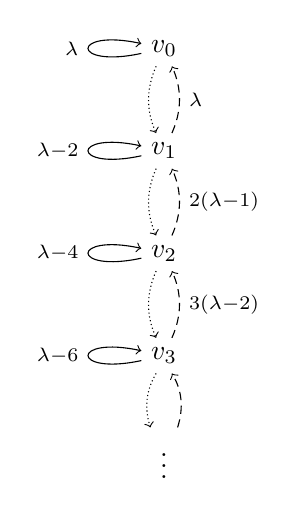
\begin{tikzpicture}[
              yscale = 1.3,
              bendy/.style = {bend right = 30},
              loopy/.style = {out = 190, in = 170, looseness = 30}
            ]
            % nodes
            \node (v0)   at (0,  0) {$v_0$};
            \node (v1)   at (0, -1) {$v_1$};
            \node (v2)   at (0, -2) {$v_2$};
            \node (v3)   at (0, -3) {$v_3$};
            \node (rest) at (0, -4) {$\vdots$};
            % the action of F
            \draw[->, densely dotted] (v0) to[bendy] (v1);
            \draw[->, densely dotted] (v1) to[bendy] (v2);
            \draw[->, densely dotted] (v2) to[bendy] (v3);
            \draw[->, densely dotted] (v3) to[bendy] (rest);
            % the action of E
            \draw[->, densely dashed ] (v1)   to[bendy] node[right] {$\scriptstyle \lambda$} (v0);
            \draw[->, densely dashed] (v2)   to[bendy] node[right] {$\scriptstyle 2(\lambda-1)$} (v1);
            \draw[->, densely dashed] (v3)   to[bendy] node[right] {$\scriptstyle 3(\lambda-2)$} (v2);
            \draw[->, densely dashed] (rest) to[bendy] (v3);
            % the action of H
            \draw[->] (v0) to[loopy] node[left]{$\scriptstyle \lambda$} (v0);
            \draw[->] (v1) to[loopy] node[left]{$\scriptstyle \lambda-2$} (v1);
            \draw[->] (v2) to[loopy] node[left]{$\scriptstyle \lambda-4$} (v2);
            \draw[->] (v3) to[loopy] node[left]{$\scriptstyle \lambda-6$} (v3);
          \end{tikzpicture}
        \end{center}
        \caption{
          The Verma module~$\verma(\lambda)$ of~$\Univ(\sllie_2)$.
          The action of~$H$ is depicted by loops, the action of~$F$ by dotted arrows and the action of~$E$ by dashed arrows.
        }
        \label{graphical representation of verma module}
      \end{figure}
    \item
      The Verma module~$\verma(\lambda)$ is a representation of highest weight~$\lambda$.
    \item
      There exists for every representation~$V$ of~$\sllie_2$ an isomorphism of vector spaces given by
      \begin{align*}
        \Hom_{\sllie_2}( \verma(\lambda), V )
        &\longto
        \{
          v \in V
        \suchthat
          \text{$v$ is of weight~$\lambda$ with~$E.v = 0$}
        \} \,,
        \\
        \varphi
        &\longmapsto
        \varphi(1 \tensor 1) \,.
      \end{align*}
      In particular
      \[
        \End_{\sllie_2}( \verma(\lambda) )
        =
        \kf \,.
      \]
    \item
      The representation~$\verma(\lambda)$ is indecomposable.
    \item
      \begin{enumerate}
        \item
          If~$\lambda \notin \Natural$ then the representation~$\verma(\lambda)$ is irreducible.
        \item
          If~$\lambda = n \in \Natural$ then the representation~$\verma(\lambda)$ has a unique nonzero, proper subrepresentation, which is spanned by the vectors
          \[
            v_i
            \qquad
            \text{with~$i \geq n+1$.}
          \]
          This subrepresentation is isomorphic to~$\verma(-n-2)$.
      \end{enumerate}
  \end{enumerate}
\end{proposition}

\begin{definition}
  Let~$\lambda \in \kf$.
  \begin{enumerate}
    \item
      For~$\lambda \notin \Natural$ let~$\irred(\lambda) \defined \verma(\lambda)$.
    \item
      For~$\lambda \in \Natural$ let~$\irred(\lambda) \defined \verma(\lambda)/N$ where~$N$ is the unique nonzero, proper subrepresentation of~$\verma(\lambda)$.
  \end{enumerate}
\end{definition}

\subsubsection{Classifications of Certain Irreducible Representations}

\begin{theorem}
  \leavevmode
  \begin{enumerate}
    \item
      There is a one-to-one correspondence given by
      \begin{align*}
        \left\{
          \begin{tabular}{@{}l@{}}
            irreducible highest weight\\
            representations of~$\sllie_2$
          \end{tabular}
        \right\}
        &\longleftrightarrow
        \kf \,,
        \\
        \irred(\lambda)
        &\longmapsfrom
        \lambda \,.
      \end{align*}
    \item
      The representation~$\irred(\lambda)$ is finite-dimensional if and only if~$\lambda = n \in \Natural$, in which case
      \[
        \dim(\irred(n))
        =
        n + 1 \,.
      \]
      If~$\kf$ is algebraically closed (so that every irreducible finite-dimensional~\representation{$\sllie_2$} is a highest-weight representation) then the above correspondence does therefore restrict to a one-to-one correspondence
      \begin{align*}
        \left\{
          \begin{tabular}{@{}l@{}}
            irreducible finite-dimensional\\
            representations of~$\sllie_2$
          \end{tabular}
        \right\}
        &\longleftrightarrow
        \Natural \,,
        \\
        L
        &\longmapsto
        \dim(L) - 1 \,,
        \\
        \irred(n)
        &\longmapsfrom
        n \,.
      \end{align*}
  \end{enumerate}
\end{theorem}

\begin{remark}
  Let~$n \in \Natural$.
  The basis~$v_0, \dotsc, v_n$ of~$\irred(n)$ can be rescaled to the basis
  \[
    w_i
    \defined
    \frac{v_i}{i!} \,.
  \]
  The actions of~$E$ and~$F$ then become
  \[
    E.w_i = (n-i+1) w_{i-1} \,,
    \quad
    F.w_i = (i+1) w_{i+1} \,.
  \]
  The actions of~$E$,~$H$,~$F$ on~$\irred(n)$ can now be graphically be represented as in \cref{graphical representation of irreducible representation}.
%  \begin{figure}
%    \begin{center}
%      \begin{tikzpicture}[
%          yscale = 1.3,
%          bendy/.style = {bend right = 25},
%          loopy/.style = {out = 190, in = 170, looseness = 40}
%        ]
%        % nodes
%        \node (w0)   at (0,  0) {$w_0$};
%        \node (w1)   at (0, -1) {$w_1$};
%        \node (w2)   at (0, -2) {$w_2$};
%        \node (rest) at (0, -3) {$\vdots$};
%        \node (wn-2) at (0, -4) {$w_{n-2}$};
%        \node (wn-1) at (0, -5) {$w_{n-1}$};
%        \node (wn)   at (0, -6) {$w_n$};
%        % the action of h
%        \draw[->] (w0)    to[loopy] node[left]{$\scriptstyle n$} (w0);
%        \draw[->] (w1)    to[loopy] node[left]{$\scriptstyle n-2$} (w1);
%        \draw[->] (w2)    to[loopy] node[left]{$\scriptstyle n-4$} (w2);
%        \draw[->] (wn-2)  to[loopy, looseness = 22.5] node[left]{$\scriptstyle -n+4$} (wn-2);
%        \draw[->] (wn-1)  to[loopy, looseness = 22.5] node[left]{$\scriptstyle -n+2$} (wn-1);
%        \draw[->] (wn)    to[loopy] node[left]{$\scriptstyle -n$} (wn);
%        % the action of f
%        \draw[->, densely dotted] (w0)    to[bendy] node[left] {$\scriptstyle 1$} (w1);
%        \draw[->, densely dotted] (w1)    to[bendy] node[left] {$\scriptstyle 2$} (w2);
%        \draw[->, densely dotted] (w2)    to[bendy] (rest);
%        \draw[->, densely dotted] (rest)  to[bendy] (wn-2);
%        \draw[->, densely dotted] (wn-2)  to[bendy] node[left] {$\scriptstyle n-1$} (wn-1);
%        \draw[->, densely dotted] (wn-1)  to[bendy] node[left] {$\scriptstyle n$} (wn);
%        % the action of e
%        \draw[->, densely dashed] (w1)    to[bendy] node[right] {$\scriptstyle n$} (w0);
%        \draw[->, densely dashed] (w2)    to[bendy] node[right] {$\scriptstyle n-1$} (w1);
%        \draw[->, densely dashed] (rest)  to[bendy] (w2);
%        \draw[->, densely dashed] (wn-2)  to[bendy] (rest);
%        \draw[->, densely dashed] (wn-1)  to[bendy] node[right] {$\scriptstyle 2$} (wn-2);
%        \draw[->, densely dashed] (wn)    to[bendy] node[right] {$\scriptstyle 1$} (wn-1);
%      \end{tikzpicture}
%    \end{center}
%    \caption{The irreducible representation~$\irred(n)$.}
%    \label{graphical representation of irreducible representation}
%  \end{figure}
\end{remark}

\subsubsection{Semisimplicity of Finite-Dimensional Representations}

\begin{theorem}[Weyl]
  Let~$\kf$ be algebraically closed.
  Every finite-dimensional representation of~$\sllie_2$ is semisimple.
\end{theorem}

\begin{proof}
  See~\cite[Theorem~6.3]{humphreys_lie_algebras}.
\end{proof}

\begin{corollary}
  Any finite-dimensional representation of~$\sllie_2$ admits a weight space decomposition.
  All occuring weights are integral.
  \qed
\end{corollary}

The decomposition of a finite-dimensional representation of~$\sllie_2$ into irreducible representations can be read off from its weight space decomposition.
From this the following result can be shown.

\begin{proposition}[Clebsch--Gordan]
  Let~$n$,~$m$ be natural numbers with~$n \geq m$.
  Then
  \[
    \irred(n) \tensor \irred(m)
    \cong
    \irred(n + m) \oplus \irred(n + m - 2) \oplus \dotsb \oplus \irred(n - m) \,.
  \]
\end{proposition}

\subsubsection{The General Case of Characteristic Zero}

We have above used a few times the additional assumption that~$\kf$ is algebraically closed.
We will now explain how to get rid of this assumption.
For this we first recall some standard results about semisimplicity of algebras.

\begin{lemma}
  \label{semisimplicity via faithful representation}
  Let~$\kf$ be any field and let~$V$ be a finite-dimensional~\vectorspaces{$\kf$}.
  Let~$A$ be a subalgebra of~$\End_{\kf}(V)$.
  Then~$A$ is semisimple if and only if~$V$ is semisimple as an~\module{$A$}.
\end{lemma}

\begin{proof}
  See~\cite[XVII,~\S5,~Proposition~4.7]{lang_algebra} and~\cite{stackexchange_lang_proof}, or~\cite[Proposition~5.13]{milne_lag}
\end{proof}

\begin{definition}
  The \defemph{Jacobson radical} of a ring~$R$ is the intersection of all maximal left ideal of~$R$.
  It is denoted by~$\Jac(R)$.
\end{definition}

\begin{remark}
  Let~$R$ be a ring.
  The irreducible~\modules{$R$} are up to isomorphism precisely those~\modules{$R$} of the form~$R/\mathfrak{m}$, where~$\mathfrak{m}$ is a maximal left ideal in~$R$.
  The Jacobson radical of~$R$ does therefore consists of precisely those elements of~$R$ which annihilate every irreducible~\module{$R$}.
\end{remark}

\begin{proposition}
  Let~$A$ be a finite-dimensional~\algebra{$\kf$}.
  \begin{enumerate}
    \item
      The Jacobson radical~$\Jac(A)$ is a nilpotent, two-sided ideal in~$A$.
    \item
      Every nilpotent, two-sided ideal of~$A$ is contained in the Jacobson raidcal~$\Jac(A)$.
      It is thus the unique maximal nilpotent, two-sided ideal.
    \item
      The following conditions on~$A$ are equivalent:
      \begin{enumerate}[label = \roman*.]
        \item
          The algebra~$A$ is semisimple.
        \item
          The Jacobson radical~$J(A)$ vanishes.
        \item
          The algebra~$A$ does not contain any nonzero nilpotent, two-sided ideal.
      \end{enumerate}
  \end{enumerate}
\end{proposition}

\begin{proof}
  See~\cite[\S4]{lam_first_course}.
\end{proof}

\begin{corollary}[{\cite[Proposition~5.11]{milne_lag}}]
  \label{extension of scalars for algebras reflect semisimple}
  Let~$A$ be a finite-dimensional~\algebra{$\kf$}.
  Let~$\Kf$ be a field extension of~$\kf$ and suppose that~$\Kf \tensor_{\kf} A$ is semisimple.
  Then~$A$ is semisimple.
\end{corollary}

\begin{proof}
  We find for the Jacobson radical~$\Jac(A)$ that~$\Kf \tensor \Jac(A)$ is a nilpotent, two-sided ideal of~$\Kf \tensor A$.
  It is thus contained in the Jacobson radical~$\Jac(\Kf \tensor A)$.
  This Jacobson radical vanishes because~$\Kf \tensor A$ is semisimple.
  It follows that~$\Kf \tensor \Jac(A) = 0$ and thus~$\Jac(A) = 0$.
\end{proof}

\begin{corollary}
  \label{extension of scalars reflects semisimplicity of fd representations}
  Let~$A$ be an~\algebra{$\kf$} and let~$M$ be a finite-dimensional~\module{$A$}.
  Let~$\Kf$ be a field extension of~$\kf$ and let
  \[
    A_{\Kf} \defined \Kf \tensor_{\kf} A \,,
    \quad
    M_{\Kf} \defined \Kf \tensor_{\kf} M \,.
  \]
  If~$M_{\Kf}$ is semisimple as an~\module{$A_{\Kf}$} then~$M$ is semisimple as an~\module{$A$}.
\end{corollary}

\begin{proof}
  We replace~$A$ by its image in~$\End_{\kf}(M)$ and then apply \cref{semisimplicity via faithful representation} and \cref{extension of scalars for algebras reflect semisimple}.
\end{proof}

%\begin{remark}
%  \Cref{extension of scalars reflects irreduciblity} asserts that extension of scalars reflects irreducibility of finite-dimensional modules.
%  It is generally not true that it preserves semisimplicity:
%  It may happen that~$M$ is semisimple as an~\module{$A$} but~$M_{\Kf}$ is not semisimple as an~\module{$A_{\Kf}$}.
%\end{remark}

\begin{theorem}
  Let~$\kf$ be a field of characteristic zero.
  \begin{enumerate}
    \item
      Every finite-dimensional~\representation{$\sllie_2$} is semisimple.
    \item
      Every finite-dimensional~\representation{$\sllie_2$} decomposes into weight spaces, and all occuring weights are integral.
    \item
      The irreducible finite-dimensional representations of~$\sllie_2$ are given by~$\irred(n)$ for~$n \in \Natural$.
  \end{enumerate}
\end{theorem}

\begin{proof}
  Let~$\Kf$ be an algebraic closure of~$\kf$.
  \begin{enumerate}
    \item
      We have previously seen that the assertion holds for~$\sllie_2(\Kf)$.
      We have
      \[
        \Kf \tensor \Univ(\sllie_2(\kf))
        \cong
        \Univ(\sllie_2(\Kf))
      \]
      whence the assertion follows for~$\sllie_2(\kf)$ from \cref{extension of scalars reflects semisimplicity of fd representations}.
    \item
      The assertion holds for~$\sllie_2(\Kf)$, as previously seen.
      Let~$M$ be a finite-dimensional representaion of~$\sllie_2(\kf)$.
      Then~$\Kf \tensor_{\kf} M$ is a finite-dimensional representation of~$\sllie_2(\Kf)$ and it follows that~$\Kf \tensor_{\kf} M$ decomposes into weight spaces as described.
      This means that~$\Kf \tensor_{\kf} M$ is annihilated by the element
      \[
        x \defined \prod_{j=-n}^n (H - j)
      \]
      of~$\Univ(\sllie_2(\Kf))$ for some sufficiently large~$n \geq 0$.
      It follows that~$x$, regarded as an element of~$\Univ(\sllie_2(\kf))$, annihilates the original representation~$M$.
      The assertion for~$\sllie_2(\kf)$ follows from this.
    \item
      It follows from the previous assertion that every finite-dimensional irreducible~\representation{$\sllie_2(\kf)$} is a highest-weight representations.
      The classification of irreducible, finite-dimensional highest-weight representations of~$\sllie_2$ works the same over every field of characteristic zero.
      We hence get for~$\sllie_2(\kf)$ the asserted classification.
    \qedhere
  \end{enumerate}
\end{proof}



\subsection{An Alternative Presentation for~$\Univ_q(\sllie_2)$}
\label{alternative presentation for quantum sl2}

Let~$q \in \kf$ and let~$U_q$ be the algebra given by the generators
\[
  E \,,
  \quad
  \widetilde{H} \,,
  \quad
  F \,,
  \quad
  K \,,
  \quad
  K^{-1} 
\]
and the relations
\begin{gather*}
  K K^{-1} = 1 = K^{-1} K \,,
  \quad
  KE = q^2 EK \,,
  \quad
  KF = q^{-2} FK \,,
  \\
  [E,F] = \widetilde{H} \,,
  \quad
  (q - q^{-1}) \widetilde{H} = K - K^{-1} \,,
  \\
  [\widetilde{H}, E] = q(EK + K^{-1} E) \,,
  \quad
  [\widetilde{H}, F] = -q^{-1}(FK + K^{-1} F) \,.
\end{gather*}

\begin{proposition}
  There exists a unique homomorphism of algebras
  \[
    \psi
    \colon
    U_q
    \to
    \Univ_q(\sllie_2)
  \]
  that is given by
  \[
    \psi(E) = E \,,
    \quad
    \psi(\widetilde{H}) = \frac{K - K^{-1}}{q - q^{-1}} \,,
    \quad
    \psi(F) = F \,,
    \quad
    \psi(K) = K \,,
  \]
  and this homomorphism is an isomorphism.
\end{proposition}

\begin{proof}
 See~{\cite[Proposition~VI.2.1]{kassel_quantum}}.
\end{proof}

\begin{proposition}
  For~$q = 1$ there exists a unique homomorphism of algebras
  \[
    \varphi
    \colon
    U_1
    \to
    \Univ(\sllie_2)[\sigma]/(\sigma^2 - 1)
  \]
  that is given by
  \[
    \varphi(E) = \sigma E \,,
    \quad
    \varphi(\widetilde{H}) = \sigma H \,,
    \quad
    \varphi(F) = F \,,
    \quad
    \varphi(K) = \sigma \,.
  \]
\end{proposition}

\begin{proof}
  See~\cite[Proof of Proposition~VI.2.2]{kassel_quantum}.
\end{proof}

\begin{remark}
  There also exist other, more exotic presentations of~$\Univ_q(\sllie_2)$.
  We refer to~\cite{equitable_presentation} for an example.
\end{remark}




\subsection{Representation Theory of~$\Univ_1(\sllie_2)$}
\label{representation theory of U1}

Let~$A$ denote the algebra~$\Univ(\sllie_2)[\sigma]/(\sigma^2 - 1)$.

Let~$M$ be an~\representation{$\sllie_2$} and let~$\varepsilon = \pm 1$.
The corresponding~\module{$\Univ(\sllie_2)$} structure on~$M$ extends to an~\module{$\Univ(\sllie_2)[\sigma]$} structure for which~$\sigma$ acts by multiplication with~$\varepsilon$, because~$\sigma$ is central in~$\Univ(\sllie_2)[\sigma]$.
It follows from~$\varepsilon^2 = 1$ that this induces a~\module{$A$} structure on~$M$ as claimed in \cref{quantum U1}.

If~$M$ is irreducible then the resulting~\module{$A$} is again irreducible since every~\submodule{$A$} is in particular an~\subrepresentation{$\sllie_2$}.
It hence follows that the~\modules{$A$}~$\irred(+,n)$ and~$\irred(-,n)$ that result from the irreducible~\representation{$\sllie_2$}~$\irred(n)$ are again irreducible.
These representations are pairwise non-isomorphic since the element~$H \sigma$ of~$A$ (which corresponds to the element~$\widetilde{H}$ of~$\Univ_1(\sllie_2)$) acts on~$\irred(+,n)$ with highest weight~$n$ and on~$\irred(-,n)$ with highest weight~$-n$.

Let now~$M$ be any finite-dimensional~\module{$M$}.
It follows from the relation~$\sigma^2 = 1$ in~$A$ that the action of~$\sigma$ on~$A$ is diagonalizable with eigenvalues~$1$ and~$-1$.
We thus have
\[
  M = M_{1} \oplus M_{-1}
\]
with~$M_\varepsilon \defined \{ m \in M \suchthat \sigma m = \varepsilon m \}$ for~$\varepsilon = \pm 1$.
The action of~$\sigma$ on~$M$ is an~\module{$A$} homomorphism because~$\sigma$ is central in~$A$.
The decomposition~$M = M_{1} \oplus M_{-1}$ is therefore one of~\modules{$A$}.

We may regard both~$M_1$ and~$M_{-1}$ as~\representations{$\sllie_2$} by restriction.
We then have decompositions into finite-dimensional irreducible~\representations{$\sllie_2$} given by
\[
  M_1
  \cong
  \irred(n_1) \oplus \dotsb \oplus \irred(n_s) \,,
  \quad
  M_{-1}
  \cong
  \irred(n'_1) \oplus \dotsb \oplus \irred(n'_t) \,.
\]
We note that this is already a decomposition as~\modules{$A$} since~$\sigma$ acts on~$M_1$ and~$M_{-1}$ by multiplication with scalars.
As~\modules{$A$} we have
\[
  \irred(n_i) = \irred(+, n_i) \,,
  \quad
  \irred(n'_i) = \irred(-, n'_i) \,.
\]
This shows that every finite-dimensional~\module{$A$} decomposes into a direct sum of the irreducible~\modules{$A$}~$\irred(\varepsilon, n)$.




\subsection{PBW Basis for~$\Univ_q(\sllie_2)$}
\label{proof of quantum pbw}

We use in the following the notation introduced in \cref{definition of quantum integers}.

\begin{lemma}
  \label{generalized commutator relation for E and F}
  For every~$r \geq 0$ we have
  \[
    [E, F^r]
    =
    \qnum{r} F^{r-1} \qnum{K, 1-r} \,.
  \]
\end{lemma}

\begin{proof}
  For~$r = 0$ both sides vanish and for~$r = 1$ this is one of the defining relations of~$\Univ_q(\sllie_2)$.
  For~$r \geq 2$ the assertion follows by induction, see~\cite[Appendix 1.3~(5)]{jantzen_quantum}.
\end{proof}

\begin{corollary}
  \label{technical formulas}
  We have
  \begin{align*}
    F \cdot F^l K^m E^n
    &=
    F^{l+1} K^m E^n \,,
    \\
    K^{\pm 1} \cdot F^l K^m E^n
    &=
    q^{\mp 2l} F^l K^{m \pm 1} E^n \,,
    \\
    E \cdot F^l K^m E^n
    &=
    q^{-2m} F^l K^m E^{n+1}
    +
    \frac{\qnum{l}}{q - q^{-1}}
    (
      q^{1-l} F^{l-1} K^{m + 1-l} E^n
      -
      q^{l-1} F^{l-1} K^{m + l-1} E^n
    ) \,.
  \end{align*}
\end{corollary}

\begin{proof}
  This follows from \cref{generalized commutator relation for E and F} and the two relations~$KE = q^2 EK$ and~$KF = q^{-2} FK$.
\end{proof}

\begin{proof}[Proof of \cref{quantum pbw}]
  Let~$U$ be the linear subspace of~$\Univ_q(\sllie_2)$ spanned by these given monomials. 
  It follows from \cref{technical formulas} that~$\Univ_q(\sllie_2)$ is a left ideal.
  It contains the elements~$F^0 K^0 E^0 = 1$, whence~$U = \Univ_q(\sllie_2)$.
  This shows that the given monomials are a vector space generating set.

  The linear independence is shown in the usual representation-theoretic way:
  Let~$V$ be the free vector space with basis
  \[
    X^l Y^n Z^m
    \qquad
    \text{with~$l, n \in \Natural$ and~$m \in \Integer$}.
  \]
  There exists an action of~$\Univ_q(\sllie_2)$ on~$V$ by using the formulas from \cref{technical formulas}, with~$F^l K^m E^n$ replaced by~$X^l Y^n Z^m$.
  (It has to be checked that this proposed action is compatible with the defining relations of~$\Univ_q(\sllie_2)$, see~\cite[Appendix 1.5]{jantzen_quantum}.)
  The elements
  \[
    F^l K^m E^n \cdot X^0 Y^0 Z^0
    =
    X^l Y^m Z^n
  \]
  are linearly independent in~$V$, whence the given monomials~$F^l K^m E^n$ are linearly independent in~$\Univ_q(\sllie_2)$.
\end{proof}



\subsection{More on the Algebra Structure of~$\Univ_q(\sllie_2)$}

\label{algebra structure of quantum sl2}
\begin{remark}
  \leavevmode
  \begin{enumerate}
    \item
      The universal enveloping algebra~$\Univ(\sllie_2)$ is noetherian and has no nonzero zero divisors.
      The same holds for~$\Univ_q(\sllie_2)$, see~\cite[Proposition~VI.1.4]{kassel_quantum} and~\cite[Propositon~1.8]{jantzen_quantum}.
    \item
      The algebra~$\Univ_q(\sllie_2)$ admits a grading such that~$E$,~$K$,~$F$ are homogeneous with
      \[
        \deg(E) = 1 \,,
        \quad
        \deg(F) = -1 \,,
        \quad
        \deg(K) = 0 \,.
      \]
      The degree~$d$ part of~$\Univ_q(\sllie_2)$ has the basis
      \[
        F^l K^m E^n
        \qquad
        \text{with~$n - l = d$.}
      \]
      This grading wan also be characterized in terms of the conjugation map
      \[
        \Univ_q(\sllie_2)
        \to
        \Univ_q(\sllie_2) \,,
        \quad
        x
        \mapsto
        K x K^{-1} \,.
      \]
      The degree~$d$ part of the grading is precisely the eigenspace with eigenvalue~$q^{2d}$.
  \end{enumerate}
\end{remark}

\begin{proposition}
  \leavevmode
  \begin{enumerate}
    \item
      There exists a unique algebra involution~$\omega$ of~$\Univ_q(\sllie_2)$ with
      \begin{alignat*}{3}
        \omega(E) &= F \,,
        &\quad
        \omega(K) &= K^{-1} \,,
        &\quad
        \omega(F) &= E \,.
    \intertext{
    \item
      There exists a unique algebra anti-involution~$\tau$ of~$\Univ_q(\sllie_2)$ with
    }
        \tau(E) &= E \,,
        &\quad
        \tau(K) &= K^{-1} \,,
        &\quad
        \tau(F) &= F \,.
    \intertext{
    \item
      There exists a unique algebra isomorphism~$\varphi_q \colon \Univ_q(\sllie_2) \to \Univ_{q^{-1}}(\sllie_2)$ with
    }
        \varphi(E) &= -F \,,
        &\quad
        \varphi(K) &= K^{-1}
        &\quad
        \varphi(F) &= -E \,.
    \intertext{
      The inverse of the isomorphism~$\varphi_q$ is given by~$\varphi_{q^{-1}}$.
    \item
      There exist unique algebra involutions~$\sigma_E$ and~$\sigma_F$ of~$\Univ_q(\sllie_2)$ with
    }
        \sigma_E(E) &= -E \,,
        &\quad
        \sigma_E(K) &= -K \,,
        &\quad
        \sigma_E(F) &= F \,.
    \shortintertext{and}
        \sigma_F(E) &= E \,,
        &\quad
        \sigma_F(K) &= -K \,,
        &\quad
        \sigma_E(F) &= -F \,.
    \end{alignat*}
  \end{enumerate}
\end{proposition}

\begin{proof}
  One checks that the proposed images of~$E$,~$F$,~$K^{\pm 1}$ are compatible with the defining relations of~$\Univ_q(\sllie_2)$.
  See also~\cite[Lemma~1.2]{jantzen_quantum}.
\end{proof}

\begin{remark}
  \leavevmode
  \begin{enumerate}
    \item
      One can combine the above (anti-)isomorphisms to construct further (anti-)isomorphisms involving~$\Univ_q(\sllie_2)$ and~$\Univ_{q^{-1}}(\sllie_2)$.
    \item
      It follows from the existence of these (anti-)isomorphisms that many formulas and propositions involving~$\Univ_q(\sllie_2)$ have to satisfy certain symmetries.
      % TODO: Explicit examples.
  \end{enumerate}
\end{remark}

% TODO: Explain how these isomorphisms come from isomorphisms of sl2, via formal deformations.



\subsection{Proof of \cref{quantum weight decomposition}}
\label{proof of quantum weight decomposition}

\begin{lemma}
  \label{action on finite dimensional modules}
  Let~$M$ be a finite-dimensional~\module{$\Univ_q(\sllie_2)$}.
  \begin{enumerate}
    \item
      Both~$E$ and~$F$ act nilpotently on~$M$.
    \item
      For a sufficiently large power~$r \geq 0$ (namely such that~$F^r M = 0$) the module~$M$ is annihilated by
      \[
        \prod_{j = -r}^r (K^2 - q^{2j}) \,.
      \]
  \end{enumerate}
\end{lemma}

\begin{proof}
  See~\cite[Proposition~2.1]{jantzen_quantum} and~\cite[Proposition~2.3]{jantzen_quantum}.
\end{proof}

\begin{proposition}
  Every finite-dimensional~\module{$\Univ_q(\sllie_2)$} decomposes into weight spaces.
  All occuring weights are of the form~$\pm q^n$ for some~$n \in \Integer$.
\end{proposition}

\begin{proof}
  Let~$M$ be a finite-dimensional~\module{$\Univ_q(\sllie_2)$} and let~$k$ denote the action of~$K$ on~$M$.
  It follows from \cref{action on finite dimensional modules} that
  \[
    0
    =
    \prod_{n = -r}^r ( k^2 - q^{2n} )
    =
    \prod_{n = -r}^r ( k - q^n ) ( k + q^n ) \,.
  \]
  The roots~$\pm q^n$ with~$n = -r, \dotsc, r$ are pairwise distinct%
  \footnote{
    If~$\pm q^n = \pm q^m$ then squaring both sides of this equation gives~$q^{2n} = q^{2m}$ and thus~$q^{2(n-m)} = 1$.
    It follows that~$2(n-m) = 0$ because~$q$ is not a root of unity, and thus~$n = m$.
  }
  whence it follows that~$k$ is diagonalizable with possible eigenvalues~$\pm q^n$ for~$n = -r, \dotsc, r$.
\end{proof}



\subsection{Proof of \cref{understanding quantum verma modules}}
\label{proof of understanding quantum verma modules}

\begin{proposition}
  \label{quantum borel}
  \leavevmode
  \begin{enumerate}
    \item
      The algebra~$\Univ_q(\blie)$ has the basis
      \[
        K^n E^m
        \qquad
        \text{with~$n \in \Integer$ and~$m \in \Natural$}
      \]
    \item
      The algebra~$\Univ_q(\blie)$ is given with respect to its generators~~$E$,~$K$,~$K^{-1}$ by the relations
      \[
        K K^{-1} = 1 = K^{-1} K \,,
        \quad
        K E = q^2 E K \,.
      \]
  \end{enumerate}
\end{proposition}

\begin{proof}
  \leavevmode
  \begin{enumerate}
    \item
      Let~$U$ be the linear subspace of~$\Univ_q(\sllie_2)$ spanned by the monomials~$K^n E^m$ with~$n, m \in \Natural$.
      This linear subspace is contained in~$\Univ_q(\blie)$.
      It follows on the other hand from the relation~$KE = q^2 EK$ that
      \[
        K^n E^m \cdot K^{n'} E^{m'}
        =
        q^{2 m n'} K^{n + n'} E^{m + m'}
      \]
      for all~$n, n', m, m' \in \Natural$, and we have~$1 = K^0 E^0 \in U$.
      This shows that~$U$ is a subalgebra of~$\Univ_q(\sllie_2)$ containing~$E$,~$K$,~$K^{-1}$, and therefore containing~$\Univ_q(\blie)$.
      This shows together that~$U = \Univ_q(\blie)$.
    \item
      Let~$U$ be the algebra given by generators~$E$,~$K$,~$K^{-1}$ and relations
      \[
        K K^{-1} = 1 = K^{-1} K \,,
        \quad
        KE = q^2 EK \,.
      \]
      There exists a unique algebra homomorphism~$\varphi \colon U \to \Univ_q(\blie)$ given by
      \[
        \varphi(E) = E \,,
        \quad
        \varphi(K) = K \,.
      \]
      In the same way as \cref{quantum pbw} one sees that~$U$ has a PBW-basis given by the monomials
      \[
        K^n E^m
        \qquad
        \text{with~$n \in \Integer$ and~$m \in \Natural$.}
      \]
      It follows that the algebra homomorphism~$\varphi$ restricts to a bijection between the PBW-bases of~$U$ and~$\Univ_q(\blie)$ and is therefore an algebra isomorphism.
    \qedhere
  \end{enumerate}
\end{proof}

We now show an extended version of \cref{understanding quantum verma modules}

\begin{proposition}
  Let~$\lambda \in \kf^\times$.
  \begin{enumerate}
    \item
      We have~$\kf_\lambda \cong \Univ_q(\blie) / \gen{E, K - \lambda}$ as an~\module{$\Univ_q(\blie)$}.
    \item
      The Verma module~$\verma(\lambda)$ has the basis
      \[
        m_i
        \defined
        F^i \tensor 1
        \qquad
        \text{with~$i \geq 0$,}
      \]
      and the actions of~$E$,~$K$,~$F$ on this basis is given by
      \[
        F m_i = m_{i+1} \,,
        \quad
        K m_i = q^{-2i} \lambda m_i \,,
        \quad
        E m_i = \qnum{i} \qnum{\lambda, 1-i} m_{i-1} \,.
      \]
      This action can be graphically described as in \cref{graphical representation of quantum verma module}.
    \item
      The Verma module~$\verma(\lambda)$ is of highest weight~$\lambda$, and every~\module{$\Univ_q(\sllie)$} of highest weight~$\lambda$ is a quotient of~$\verma(\lambda)$.
    \item
      There exists for every~\module{$\Univ_q(\sllie_2)$}~$M$ an isomorphism of vector spaces given by
      \[
        \Hom_{\Univ_q(\sllie_2)}( \verma(\lambda), M )
        \cong
        \{
          m \in M
        \suchthat
          \text{$m$ is of weight~$\lambda$ with~$Em = 0$}
        \} \,.
      \]
      It follows in particular that
      \[
        \End_{\Univ_q(\sllie_2)}( \verma(\lambda) )
        =
        \kf \,.
      \]
    \item
      The Verma module~$\verma(\lambda)$ is indecomposable.
    \item
      \begin{enumerate}
        \item
          If~$\lambda = \pm q^n$ for some~$n \in \Natural$ then the Verma module~$\verma(\lambda)$ contains a unique nonzero, proper submodule, which is spanned by the elements
          \[
            m_i
            \qquad
            \text{with~$i \geq n+1$.}
          \]
          This submodule is isomorphic to~$\verma(q^{-n-2} \lambda)$.
        \item
          If~$\lambda \neq \pm q^n$ for every~$n \in \Natural$ then the Verma module~$\verma(\lambda)$ is irreducible.
      \end{enumerate}
  \end{enumerate}
\end{proposition}

\begin{enumerate}
  \item
    This follows from the PBW-basis of~$\Univ_q(\blie)$.
  \item
    This follows from the PBW-basis of~$\Univ_q(\sllie_2)$ and induction.
  \item
    The Verma module~$\verma(\lambda)$ is generated by the primitive weight vector~$1 \tensor 1$.
  \item
    We have
    \begin{align*}
      \SwapAboveDisplaySkip
      \Hom_{\Univ_q(\sllie_2)}( \verma(\lambda), M )
      &\cong
      \Hom_{\Univ_q(\blie)}( \kf_\lambda, M )
      \\
      &\cong
      \Hom_{\Univ_q(\blie)}( \Univ_q(\blie) / \gen{K - \lambda, E}, M)
      \\
      &\cong
      \{
        m \in M
      \suchthat
        (K - \lambda) m = 0,
        E m = 0
      \} \,.
    \end{align*}
  \item
    The endomorphism algebra~$\End_{\Univ_q(\sllie_2)}( \verma(\lambda) ) = \kf$ does not contain any non-trivial idempotents.
  \item
    This follows as for~$\Univ(\sllie_2)$ since~$\qnum{i} \qnum{\lambda, i-1} = 0$ if and only if~$\lambda = \pm q^{i-1}$.
\end{enumerate}


\subsection{Proof of \cref{finite-dimensional quantum modules are semisimple}}
\label{proof of finite-dimensional quantum modules are semisimple}

%\begin{theorem}
%  \label{finite-dimensional quantum modules are semisimple}
%  Every finite-dimensional~\module{$\Univ_q(\sllie_2)$} is semisimple.
%\end{theorem}
%
%\begin{proof}
%  Let~$M$ be a nonzero finite-dimensional~\module{$\Univ_q(\sllie_2)$}.
%  Let~$N$ be a maximal submodule of~$M$.
%  The quotient~$L \defined M/N$ is irreducible and finite-dimensional and thus of the form~$\irred(\lambda)$.
%  From the short exact sequence
%  \begin{equation}
%    \label{short exact sequence of modules}
%    0
%    \to
%    N
%    \to
%    M
%    \to
%    \irred(\lambda)
%    \to
%    0
%  \end{equation}
%  and the equality~$\irred(\lambda)_{q^2 \lambda} = 0$ we get the following commutative diagram:
%  \[
%    \begin{tikzcd}
%      0
%      \arrow{r}
%      &
%      N_\lambda
%      \arrow{r}
%      \arrow{d}[left]{E}
%      &
%      M_\lambda
%      \arrow{r}
%      \arrow{d}[left]{E}
%      &
%      \irred(\lambda)_\lambda
%      \arrow{r}
%      \arrow{d}[left]{E}
%      &
%      0
%      \\
%      0
%      \arrow{r}
%      &
%      N_{q^2 \lambda}
%      \arrow[equal]{r}
%      &
%      M_{q^2 \lambda}
%      \arrow{r}
%      &
%      0
%      \arrow{r}
%      &
%      0
%    \end{tikzcd}
%  \]
%  Let us denote for every~\module{$\Univ_q(\sllie_2)$}~$P$ by~$P^E$ the linear subspace
%  \[
%    P^E
%    \defined
%    \{
%      p \in P
%    \suchthat
%      Ep = 0
%    \} \,.
%  \]
%  We get by the snake lemma an exact sequence
%  \[
%    0
%    \to
%    N_\lambda^E
%    \to
%    M_\lambda^E
%    \to
%    \irred(\lambda)_\lambda^E
%    \to
%    E N_{q^2 \lambda}
%    \xto{\id}
%    E M_{q^2 \lambda}
%    \to
%    0 \,.
%  \]
%  It follows from the exact sequence that the induced map~$M_\lambda^E \to \irred(\lambda)_\lambda^E$ is surjective.
%  There hence exists some element~$m \in M_\lambda^E$ that is mapped to the primitive generator~$v_0$ of~$\irred(\lambda)$.
%  There exists a module homomorphism
%  \[
%    \varphi
%    \colon
%    \verma(\lambda)
%    \to
%    M \,,
%    \quad
%    1 \tensor 1
%    \mapsto
%    m
%  \]
%  and it follows from the finite-dimensionality of~$\irred(\lambda)$ that~$\widetilde{\varphi}$ descends to a module homomorphism
%  \[
%    \psi
%    \colon
%    \irred(\lambda)
%    \to
%    M \,,
%    \quad
%    v_0
%    \mapsto
%    m \,.
%  \]
%  This shows that the short exact sequence~\eqref{short exact sequence of modules} splits, whence
%  \[
%    M
%    \cong
%    N \oplus \irred(\lambda) \,.
%  \]
%  We now proceed by induction.
%\end{proof}

\begin{lemma}
  \label{endomorphism of highest weight is ground field}
  If~$M$ is an highest-weight~\module{$\Univ_q(\sllie_2)$} then
  \[
    \End_{\Univ_q(\sllie_2)}(M) = \kf \,.
  \]
\end{lemma}

\begin{definition}
  The \defemph{quantum Casimir element} is the element~$C_q \in \Univ_q(\sllie_2)$ given by
  \[
    C_q
    \defined
    EF + \frac{ K q^{-1} + K^{-1} q }{ (q - q^{-1})^2 } \,.
  \]
\end{definition}

\begin{lemma}
  \label{action of the quantum casimir element}
  \leavevmode
  \begin{enumerate}
    \item
      The element~$C_q$ is central in~$\Univ_q(\sllie_2)$.
    \item
      The element~$C_q$ acts on every~\module{$\Univ_q(\sllie_2)$} by module endomorphisms.
    \item
      The element~$C_q$ acts for every scalar~$\lambda \in \kf^\times$ on the representation~$\irred(\lambda)$ by multiplication with the scalar
      \[
        \frac{\lambda q + \lambda^{-1} q^{-1}}{ (q - q^{-1})^2 } \,.
      \]
    \item
      The element~$C_q$ acts the same on~$\irred(\lambda)$ and~$\irred(\mu)$ if and only if~$\lambda = \mu$ or~$\lambda = \mu^{-1} q^{-2}$.
  \end{enumerate}
\end{lemma}

\begin{proof}
  \leavevmode
  \begin{enumerate}
    \item
      It can be checked that~$C_q$ commutes with~$E$,~$F$,~$K$ by using the defining relations for~$\Univ_q(\sllie_2)$.
    \item
      This follows from the previous assertion.
    \item
 
     It follows from the previous assertion and \cref{endomorphism of highest weight is ground field} that~$C_q$ acts by a scalar.
      This scalar can be read off from the action on the primitive generator~$1 \tensor 1$.
      It thus sufficies to show the assertion for~$\verma(\lambda)$, where it follows from \cref{understanding quantum verma modules}.
    \item
      This follows from the previous assertion.
    \qedhere
  \end{enumerate}
\end{proof}

\begin{corollary}
  \label{quantum casimir acts by different scalars}
  The quantum Casimir element~$C_q$ acts on every finite-dimensional, irreducible representation of~$\Univ_q(\sllie_2)$ by a different scalar.
\end{corollary}

\begin{proof}
  If~$\lambda = \delta q^n$ and~$\mu = \varepsilon q^m$ with~$\delta, \varepsilon \in \{1, -1\}$ and~$n, m \in \Natural$ then it cannot happen that~$\lambda = \mu^{-1} q^{-2}$.
  The assertion thus follows from \cref{action of the quantum casimir element}.
\end{proof}

\begin{proof}[Proof of \cref{finite-dimensional quantum modules are semisimple} ({\cite[Theorem~2.9]{jantzen_quantum}})]
  Let~$M$ be any finite-dimensional~\module{$\Univ_q(\sllie_2)$} and let~$c$ denote the action of~$C_q$ on~$M$.
  We may assume that~$M$ is indecomposable.
  We can consider a composition series
  \begin{equation}
    \label{composition series}
    0
    =
    M_0
    \subsetneq
    M_1
    \subsetneq
    M_2
    \subsetneq
    \dotsb
    \subsetneq
    M_r
    =
    M
  \end{equation}
  with composition factors
  \[
    M_i/M_{i-1}
    \cong
    \irred(\varepsilon_i q^{n_i}) \,.
  \]
  Letting~$c_i$ be the scalar by which~$C_q$ acts on~$\irred(\varepsilon_i q^{n_i})$, we have
  \[
    (c - c_i) M_i \subseteq M_{i-1} \,.
  \]
  It follows that~$\prod_{i=1}^r (c - c_i)$ annihilates~$M$ and that~$c$ admits a generalized eigenspace decomposition with eigenvalues~$c_1, \dotsc, c_r$.
  The resulting generalized eigenspaces are subrepresentations because~$c$ is a~\module{$\Univ_q(\sllie_2)$} endomorphism.
  It follows that
  \[
    c_1 = \dotsb = c_r
  \]
  because~$M$ is indecomposable, and thus
  \[
    \varepsilon_1 q^{n_1}
    =
    \dotsb
    =
    \varepsilon_r q^{n_r}
    \defines
    \lambda
  \]
  by \cref{quantum casimir acts by different scalars}.
  It follows with the composition series~\eqref{composition series} that
  \[
    \dim( M_\mu )
    =
    r \dim( \irred(\lambda)_\mu )
  \]
  for every scalar~$\mu \in \kf^\times$.
  Thus~$M$ is of highest weight~$\lambda$.

  The short exact sequence
  \begin{equation}
    \label{short exact sequence of quantum modules}
    0
    \to
    M_{r-1}
    \to
    M
    \to
    \irred(\lambda)
    \to
    0
  \end{equation}
  restricts to a short exact sequence
  \[
    0
    \to
    ( M_{r-1} )_\lambda
    \to
    M_\lambda
    \to
    \irred(\lambda)_\lambda
    \to
    0 \,.
  \]
  It follows that the primitive generator~$v_0$ of~$\irred(\lambda)$ has a preimage~$m_0$ in~$M$.
  The weight vector~$m_0$ is primitive because~$M$ isof highest weight~$\lambda$.
  It follows that there exists a homomorphism of~\modules{$\Univ_q(\sllie_2)$}
  \[
    \varphi
    \colon
    \verma(\lambda)
    \to
    M
    \,,
    \quad
    1 \tensor 1
    \mapsto
    m_0 \,.
  \]
  It follows from the finite-dimensionality of~$M$ that~$\varphi$ factors through a homomorphism
  \[
    \psi
    \colon
    \irred(\lambda)
    \to
    M
    \,,
    \quad
    \class{1 \tensor 1}
    \mapsto
    m_0 \,.
  \]
  This shows that the short exact sequence~\eqref{short exact sequence of quantum modules} splits, whence
  \[
    M \cong M_{r-1} \oplus \irred(\lambda) \,.
  \]
  It follows by induction that~$M_{r-1} \cong \irred(\lambda)^{\oplus (r-1)}$ and thus altogether~$M \cong \irred(\lambda)^{\oplus r}$.
\end{proof}

\begin{remark}
  The center of the universal enveloping algebra~$\Univ(\sllie_2)$ is a polynomial algebra, generated by the classical Casimir element~$C = (ef + h^2 + fe)/4$.
  It can be shown that the center of~$\Univ_q(\sllie_2)$ is again a polynomial algebra, now generated by the quantum Casimir element~$C_q$.
  We refer to~\cite[Proposition~2.18]{jantzen_quantum} for more details on this.
\end{remark}



\subsection{Proof of \cref{quantum weight spaces of tensor product}}
\label{proof of quantum weight spaces of tensor product}

We have
\[
  M_\mu \tensor N_\kappa
  \subseteq
  (M \tensor N)_{\mu \kappa}
\]
for all~$\mu, \kappa \in \kf^\times$ since the element~$K$ is group-like in~$\Univ_q(\sllie_2)$.
Both~$M$ and~$N$ admits weight space decompositions
\[
  M = \bigoplus_\mu M_\mu \,,
  \quad
  N = \bigoplus_\kappa N_\kappa
\]
and it follows that
\[
  M \tensor N
  =
  \biggl( \bigoplus_\mu M_\mu  \biggr)
  \tensor
  \biggl( \bigoplus_\kappa N_\kappa  \biggr)
  =
  \bigoplus_{\mu, \kappa} (M_\mu \tensor N_\kappa)
  \subseteq
  \bigoplus_{\lambda} M_{\lambda}
  \subseteq
  M \tensor N
\]
It folllows with the inclusions~$M_\mu \tensor N_\kappa \subseteq (M \tensor N)_{\mu \kappa}$ that already
\[
  (M \tensor N)_{\lambda}
  =
  \bigoplus_{\mu \kappa = \lambda}
  M_\mu \tensor N_\kappa
\]
for every~$\lambda$.



\subsection{Clebsch--Gordan for~$\Univ_q(\sllie_2)$}
\label{quantum clebsch gordan}

\begin{proposition}
  For all~$\delta, \varepsilon \in \{1, -1\}$ and~$n, m \in \Natural$ with~$n \geq m$ we have
  \[
    \irred(\delta q^n) \tensor \irred(\varepsilon q^m)
    \cong
    \irred(\delta \varepsilon q^{n+m})
    \oplus
    \irred(\delta \varepsilon q^{n+m-2})
    \oplus
    \dotsb
    \oplus
    \irred(\delta \varepsilon q^{n-m}) \,.
  \]
\end{proposition}

\begin{proof}
  This follows from \cref{decomposition from quantum weight spaces} and \cref{quantum weight spaces of tensor product}.
\end{proof}





\section{Deformation Theory}
\label{deformation theory}



\subsection{Deformations of Algebras}

We will in the following introduce a formal deformation~$\Univ_{\hbar}(\sllie_2)$ of the Hopf algebra~$\Univ(\sllie_2)$ and gain a new understanding of~$\Univ_q(\sllie_2)$.



\subsection{Deformation of Algebras}

The following is taken (at least in spirit) from~\cite[\S 5.2]{pieter_hochschild} and~\cite{gerstenhaber_quantum}.

\begin{motivation}
  Deforming a~\algebra{$\kf$}~$A$ means -- roughly speaking -- that the multiplication on~$A$ is replaced by a perturbated multiplication~$*$, in the sense that for all~$a, b \in A$,
  \[
    a * b
    =
    ab + \mu_1(a,b) \hbar + \mu_2(a,b) \hbar^2 + \dotsb
  \]
  for some bilinear terms~$\mu_i(a,b)$.
  The limit~$\hbar \to 0$ does then give back the original algebra~$A$.
\end{motivation}

\begin{definition}
  \label{definition of algebra deformations}
  Let~$A$ be an~\algebra{$\kf$}.
  \begin{enumerate}
    \item
      A \defemph{(formal) deformation} of~$A$ is an~\algebra{$\kfhbar$}~$A_\hbar$ whose underlying~\module{$\kfhbar$} is~$\power{A}{\hbar}$ and for which~$A_\hbar / \hbar A_\hbar = A$ as algebras.
    \item
      Two deformations~$A_\hbar$ and~$A'_\hbar$ of the algebra~$A$ are \defemph{equivalent} if there exists an isomorphism of~\algebras{$\kfhbar$}
      \[
        \varphi
        \colon
        A_\hbar
        \to
        A'_\hbar
      \]
      such that the induced isomorphism of~\algebras{$\kf$}
      \[
        A
        =
        A_\hbar / \hbar A_\hbar
        \to
        A'_\hbar / \hbar A'_\hbar
        = A
      \]
      is the identity on~$A$, i.e.
      \[
        \varphi \equiv \id_A
        \pmod{\hbar} \,.
      \]
    \item
      A deformation is \defemph{trivial} if it is equivalent to the trivial deformation (i.e. equivalent to the algebra of power series~$\power{A}{\hbar}$).
  \end{enumerate}
\end{definition}

\begin{remark}
  Every~\bilinear{$\kfhbar$} multiplication
  \[
    (-) * (-)
    \colon
    \power{A}{\hbar} \times \power{A}{\hbar}
    \to
    \power{A}{\hbar} \,.
  \]
  satisfies the equality
  \[
    \Biggl( \sum_{i=0}^\infty a_i \hbar^i \Biggr)
    *
    \Biggl( \sum_{j=0}^\infty b_j \hbar^j \Biggr)
    =
    \sum_{i,j = 0}^\infty (a_i * b_j) \hbar^{i+j} \,.
  \]
  The multiplication~$*$ can therefore be characterized by the~\bilinear{$\kf$} maps~$\mu_i \colon A \times A \to A$ such that
  \[
    a * b
    =
    \mu_0(a, b) + \mu_1(a, b) \hbar + \mu_2(a, b) \hbar^2 + \dotsb
  \]
  The condition~$\power{A}{\hbar} / \hbar \power{A}{\hbar} = A$ means that~$\mu_0$ is the original multiplication on~$A$, whence
  \[
    a * b
    =
    ab + \mu_1(a, b) \hbar + \mu_2(a, b) \hbar^2 + \dotsb
  \]
  That the multiplication~$*$ is associative gives certain compatibility conditions on the~$\mu_1$, which we won’t discuss here.
\end{remark}

\begin{example}
  Every~\algebra{$\kf$}~$A$ admits the \defemph{trivial deformation}~$\power{A}{\hbar}$ (i.e.\ the algebra of power series with its usual product).
  It corresponds to the choice~$\mu_1, \mu_2, \dotsc = 0$.
\end{example}

\begin{theorem}
  \label{existence of Uhsl2}
  The universal enveloping algebra~$\Univ(\sllie_2)$ admits a deformation with
  \begin{equation}
    \label{relations for quantum sl2}
    [H, E] = 2E \,,
    \quad
    [H, F] = -2F \,,
    \quad
    [E, F]
    =
    \frac{ \e^{\hbar H} - \e^{-\hbar H} }{ \e^{\hbar} - \e^{-\hbar} }
  \end{equation}
\end{theorem}

\begin{proof}[Proof (sketch)]
  Let~$P$ be the free algebra on the generators~$E$,~$H$,~$F$.
  Let~$I$ be the two-sided ideal in~$\power{P}{\hbar}$ given by the relations~\eqref{relations for quantum sl2}.
  Let~$J$ be the closure of~$I$ in the~\adic{$\hbar$} topology.
  Then~$J$ is again a two-sided ideal in~$\power{P}{\hbar}$.
  The described deformation can be realized as the quotient~$\power{P}{\hbar} / J$.
  We refer to~\cite[Definition-Proposition~6.4.3~ff.]{guide_to_quantum_groups} for the specific details.
\end{proof}

\begin{definition}
  The deformation of~$\Univ(\sllie_2)$ from \cref{existence of Uhsl2} is denoted by~$\Univ_{\hbar}(\sllie_2)$.
\end{definition}

\begin{remark}
  \item
    In the algebra~$\Univ_{\hbar}(\sllie_2)$ we can consider the well-defined elements
    \[
      q \defined \e^{\hbar} \,,
      \quad
      K \defined \e^{\hbar H} \,.
    \]
    The elements~~$q$,~$E$,~$F$,~$K$,~$K^{-1}$ satisfy the defining relations of~$\Univ_q(\sllie_2)$.

    Let us consider the field of Laurent polynomials~$\lpower{\kf}{\hbar}$ and the extension of scalars
    \[
      \lpower{\kf}{\hbar} \tensor_{\kfhbar} \Univ_{\hbar}(\sllie_2) \,,
    \]
    which is given as an~\module{$\lpower{\kf}{\hbar}$} by
    \[
      \lpower{\kf}{\hbar} \tensor_{\kfhbar} \Univ_{\hbar}(\sllie_2)
      =
      \kfhbar[\hbar^{-1}] \tensor_{\kfhbar} \power{\Univ(\sllie_2)}{\hbar}
      \cong
      \power{\Univ(\sllie_2)}{\hbar}[\hbar^{-1}]
      \cong
      \lpower{\Univ(\sllie_2)}{\hbar} \,.
    \]
    The field~$\lpower{\kf}{\hbar}$ contains the subfield~$\kf(q)$, and we get from the above observation an homomorphism of~\algebras{$\kf(q)$}
    \[
      \Univ_q(\sllie_2)
      \to
      \lpower{\kf}{\hbar} \tensor_{\kfhbar} \Univ(\sllie_2)
    \]
    where~$\Univ_q(\sllie_2)$ is defined over~$\kf(q)$.
  \item
    In~$\Univ_{\hbar}(\sllie_2)$ we have both the element~$H$ and the element
    \[
      \widetilde{H}
      =
      \frac{K - K^{-1}}{q - q^{-1}} \,,
    \]
    which is of the form
    \[
      \widetilde{H}
      =
      H + \text{terms of order~$\hbar^2$} \,.
    \]
    We may think about~$\widetilde{H}$ is a deformation of~$H$ (in an informal sense).
    We note that
    \[
      q \equiv 1 \,,
      \quad
      K \equiv 1 \,,
      \quad
      \widetilde{H} \equiv H
      \qquad
      \pMod{\hbar}.
    \]
\end{remark}

\begin{definition}
  The deformation of~$\Univ(\sllie_2)$ from \cref{existence of Uhsl2} is denoted by~$\Univ_{\hbar}(\sllie_2)$.
\end{definition}

\begin{remark}
  In the algebra~$\Univ_{\hbar}(\sllie_2)$ we can consider the well-defined elements
  \[
    q \defined \e^{\hbar} \,,
    \quad
    K \defined \e^{\hbar H} \,.
  \]
  The elements~$E$,~$F$,~$K$,~$K^{-1}$ satisfy the defining relations of~$\Univ_q(\sllie_2)$ and one should think about the algebra~$\Univ_q(\sllie_2)$ as somewhat of a subalgebra of~$\Univ_{\hbar}(\sllie_2)$.
  %TODO: Make this more precise: Realize U_q(sl2) as a subalgebra of C((h)) ⊗ U_h(sl_2).

  In~$\Univ_{\hbar}(\sllie_2)$ we have both the element~$H$ and the element
  \[
    \widetilde{H}
    =
    \frac{K - K^{-1}}{q - q^{-1}} \,,
  \]
  which is of the form
  \[
    \widetilde{H}
    =
    H + \text{terms of order~$\hbar^2$} \,.
  \]
  We may think about~$\widetilde{H}$ is a deformation of~$H$ (in an informal sense).
  We note that
  \[
    q \equiv 1 \,,
    \quad
    K \equiv 1 \,,
    \quad
    \widetilde{H} \equiv H
    \qquad
    \pMod{\hbar}.
  \]
\end{remark}

\begin{remark}
  One can study the deformation theory of an~\algebra{$\kf$} via homological algebra:
  The \defemph{Hochschild cochain complex} of~$A$ is given by
  \[
    \CHoch^n(A)
    \defined
    \Hom_{\kf}(A^{\tensor n}, A)
  \]
  together with certain differentials.
  The cohomology of this chain complex is the \defemph{Hochschild cohomology} of~$A$, which is denoted by
  \[
    \HH^n(A)
    \defined
    \Homology^n\bigl( \CHoch^\bullet \bigr) \,.
  \]
  One of the connections between deformation theory and Hochschild cohomology is that in the case of
  \[
    \HH^2(A) = 0
  \]
  every deformation of~$A$ is trivial.
\end{remark}

\begin{warning}
  Let~$A_\hbar$ be a deformation of an~\algebra{$\kf$}~$A$ with~$\HH^2(A) = 0$.
  The above criterion shows that~$A_\hbar$ is equivalent to~$\power{A}{\hbar}$, but it does not provide an explicit isomorphism.
\end{warning}

\begin{example}
  Let~$\glie$ be a semisimple Lie algebra.
  It can be shown that
  \[
    \HH^2( \Univ(\glie) ) = 0,
  \]
  see~\cite[Theorem~2]{gerstenhaber_quantum} or~\cite[Exercise~2.8.1,~Bonus]{schedler_nca}.
  Therefore all deformations of~$\Univ(\glie)$ (as an algebra) are trivial.

  It follows in particular that the every algebra deformation of~$\Univ(\sllie_2)$ is trivial.
  An explicit equivalence between~$\Univ_{\hbar}(\sllie_2)$ and~$\power{\Univ(\sllie_2)}{\hbar}$ is constructed in~\cite[Proposition~4.6.4]{guide_to_quantum_groups}.
\end{example}





\subsection{Background on Completions}

We also want define coalgebras (and bialgebras and Hopf algebras).
For this we need to make sense of power series in tensor products~$\power{A}{\hbar} \tensor \power{A}{\hbar}$, which does in general not make sense.
This problem is solved by using the \defemph{completed tensor product}.

\begin{definition}
  Let~$M$ be an~\module{$\kfhbar$}.
  \begin{enumerate}
    \item
      The~\defemph{\adic{$\hbar$} completion} of~$M$ is the~\module{$\kfhbar$}
      \[
        \widehat{M}
        \defined
        \lim_{n \geq 0} (M / \hbar^{n+1} M)
        =
        \left\{
          (m_n)_{n \geq 0}
        \suchthat*
          \begin{tabular}{@{}l@{}}
            $m_n \in M/ \hbar^{n+1} M$ with \\
            $m_{n+1} \equiv m_n \pMod{\hbar^{n+1}}$ for every~$n \geq 0$
          \end{tabular}
        \right\} \,.
      \]
    \item
      The \defemph{canonical homomorphism}~$M \to \widehat{M}$ is given by~$m \mapsto (\overline{m}, \overline{m}, \dotsc)$.
    \item    
      A~\module{$\kfhbar$}~$M$ is \defemph{complete} if the canonical homomorphism~$M \to \widehat{M}$ is an isomorphism.
  \end{enumerate}
\end{definition}

\begin{remark}
  \leavevmode
  \begin{enumerate}
    \item
      More explicitely, an~\module{$\kfhbar$}~$M$ is complete if and only if there exists for every sequence~$m_0, m_1, \dotsc$ of elements~$m_n \in M$ with
      \begin{alignat*}{2}
        m_{n+1} &\equiv m_n
        \pMod{\hbar^{n+1}}
        &
        \qquad
        &\text{for every~$n \geq 0$}
      \intertext{a unique element~$m \in M$ with}
        m &\equiv m_n
        \pMod{\hbar^{n+1}}
        &
        \qquad
        &\text{for every~$n \geq 0$.}
      \end{alignat*}
    \item
      Let~$M$ be a complete~\module{$\kfhbar$}
      Every sequence~$(m_i)_{i \geq 0}$ of elements~$m_i \in M$ defines a sequence~$(s_n)_{n \geq 0}$ of partial sums
      \[
        s_n
        \defined
        \sum_{i=0}^n \hbar^i m_i \,.
      \]
      for every~$n \geq 0$.
      By the completeness of~$M$ there exists a unique element~$\sum_{i=0}^\infty \hbar^i m_i$ of~$M$ with
      \[
        \sum_{i=0}^\infty \hbar^i m_i
        \equiv
        \sum_{i=0}^n \hbar^i m_i
        \pmod{\hbar^{n+1}}
        \qquad
        \text{for every~$n \geq 0$.}
      \]
  \end{enumerate}
\end{remark}

\begin{example}
  \leavevmode
  \begin{enumerate}
    \item
      Every finite-dimensional~\module{$\kfhbar$}~$M$ is complete since~$\hbar^n M = 0$ for some sufficiently large power~$n$.
    \item
      For every~\vectorspace{$\kf$} the resulting~\module{$\kfhbar$}~$\power{V}{\hbar}$ is complete.
      For every sequence of elements~$v_0, v_1, \dotsc \in V$ we have
      \[
        \sum_{i=0}^\infty \hbar^i v_i
        =
        \sum_{i=0}^\infty v_i \hbar^i \,.
      \]
  \end{enumerate}
\end{example}

\begin{proposition}
  Let~$M$,~$N$ be two~\modules{$\kfhbar$}.
  \begin{enumerate}
    \item
      For every homomorphism of~\module{$\kfhbar$}~$f \colon M \to N$ there exists a unique module homomorphism~$\widehat{f} \colon \widehat{M} \to \widehat{N}$ that makes the following square diagram commute:
      \[
        \begin{tikzcd}
          \widehat{M}
          \arrow{r}[above]{\widehat{f}}
          &
          \widehat{N}
          \\
          M
          \arrow{u}
          \arrow{r}[above]{f}
          &
          N
          \arrow{u}
        \end{tikzcd}
      \]
      The homomorphism~$\widehat{f}$ is given by
      \[
        \widehat{f} \, \Bigl( (\overline{m_0}, \overline{m_1}, \dotsc) \Bigr)
        =
        \Bigl( \overline{f(m_0)}, \overline{f(m_1)}, \dotsc \Bigr) \,.
      \]
    \item
      The assignment~$\widehat{(-)}$ defines a functor
      \[
        \widehat{(-)}
        \colon
        \Mod{\kfhbar}
        \to
        \Mod{\kfhbar} \,.
      \]
    \item
      If~$M$,~$N$ are complete then
      \[
        f\Biggl( \sum_{i=0}^\infty \hbar^i m_i \Biggr)
        =
        \sum_{i=0}^\infty \hbar^i f(m_i)
      \]
      for every sequence of elements~$m_0, m_1, \dotsc, \in M$.
    \item
      If~$N$ is complete then every homomorphism~$M \to N$ extends uniquely to a homomorphism~$\widehat{M} \to N$.
      \[
        \begin{tikzcd}
          \widehat{M}
          \arrow[dashed]{r}[above]{\exists!}
          &
          N
          \\
          M
          \arrow{u}
          \arrow{ur}
          &
          {}
        \end{tikzcd}
      \]
    \item
      If~$V$ is any~\vectorspace{$\kf$} and~$N$ is complete then every~\linear{$\kf$} map~$f \colon V \to N$ extends uniquely to a~\linear{$\kfhbar$} linear map~$f' \colon \power{V}{\hbar} \to N$.
      \[
        \begin{tikzcd}
          \power{V}{\hbar}
          \arrow[dashed]{r}[above]{\exists!}
          &
          N
          \\
          V
          \arrow{u}
          \arrow{ur}
          &
          {}
        \end{tikzcd}
      \]
      The homomorphism~$f'$ is given by
      \[
        f'\Biggl( \sum_{i=0}^\infty \hbar^i v_i \Biggr)
        =
        \sum_{i=0}^\infty \hbar^i f(v_i) \,.
      \]
    \item
      The canonical homomorphism~$M \to \widehat{M}$ induces an isomorphism of~\vectorspaces{$\kf$}
      \[
        M / \hbar M
        \longto
        \widehat{M} / \hbar \widehat{M} \,.
      \]
  \end{enumerate}
\end{proposition}

% TODO: Add a proof.

\begin{remark}
  Let~$M$ be a~\module{$\kfhbar$}.
  There exists a unique topology on~$M$ for which a basis is given by the sets
  \[
    m + \hbar^{n+1} M
  \]
  with~$m \in M$ and~$n \geq 0$.
  This topology is the~\defemph{\adic{$\hbar$} topology} on~$M$.
  It makes~$\kfhbar$ into a topological ring and every~\module{$\kfhbar$} into a topological~\module{$\kfhbar$}.
  The completion~$\widehat{M}$ is then the usual topological completion of~$M$.
\end{remark}

% TODO: Explain the topological aspects of completion more.

\begin{definition}
  Let~$M$,~$N$ be two~\modules{$\kfhbar$}.
  The \defemph{completed tensor product}
  \[
    M \ctensor N
  \]
  is the~\adic{$\hbar$} completion of the tensor product~$M \tensor_{\kfhbar} N$.
\end{definition}

\begin{proposition}
  Let~$V$,~$W$ be two~\vectorspaces{$\kf$}.
  Then the~\linear{$\kfhbar$} map
  \[
    \power{V}{\hbar} \tensor_{\kfhbar} \power{W}{\hbar}
    \to
    \power{(V \tensor W)}{\hbar} \,,
    \quad
    \Biggl( \sum_{i=0}^\infty v_i \hbar^i \Biggr)
    \tensor
    \Biggl( \sum_{j=0}^\infty w_j \hbar^j \Biggr)
    \mapsto
    \sum_{i,j=0}^\infty (v_i \tensor w_j) \hbar^{i+j}
  \]
  extends along the canonical homomorphism
  \[
    V \tensor W \to V \ctensor W
  \]
  to an isomorphism of~\modules{$\kfhbar$}
  \[
    \power{V}{\hbar} \ctensor \power{W}{\hbar}
    \to
    \power{(V \tensor W)}{\hbar} \,.
  \]
\end{proposition}

% TODO: Add a proof in the appendix.



\subsection{Deformation of Hopf Algebras}

The following is taken mostly from~\cite[Chapter~6]{guide_to_quantum_groups}.

\begin{definition}
  \label{topological definitions}
  \begin{enumerate}
    \leavevmode
    \item
      A \defemph{topological Hopf algebra} consists of a complete~\module{$\kfhbar$}~$A$ together with~\linear{$\kfhbar$} maps
      \[
        m \colon A \ctensor A \to A \,,
        \quad
        u \colon \kfhbar \to A \,,
        \quad
        \Delta \colon A \to A \ctensor A \,,
        \quad
        \varepsilon \colon A \to \kfhbar \,,
        \quad
        S \colon A \to A
      \]
      such that the usual Hopf algebra diagrams commute.
    \item
      The terms \defemph{topological algebra},~\defemph{topological coalgebra} and~\defemph{topological bialgebra} are defined analogous to topological Hopf algebras.
  \end{enumerate}
\end{definition}

\begin{remark}
  \leavevmode
  \begin{enumerate}
    \item
      A topological Hopf algebra~$A$ is generally not an actual Hopf algebra, since the comultiplication
      \[
        \Delta
        \colon
        A
        \to
        A \ctensor A
      \]
      does in general not restrict to a map~$A \to A \tensor A$.
    \item
      If~$A$ is a topological Hopf algebra then~$A / \hbar A$ becomes an Hopf algebra over~$\kf$.
      We note for this that
      \[
        (A \ctensor A) / \hbar (A \ctensor A)
        \cong
        (A \tensor A) / \hbar (A \tensor A)
        \cong
        (A / \hbar A) \tensor (A / \hbar A) \,.
      \]
  \end{enumerate}
\end{remark}

\begin{remark}
  A topological algebra in the sense of \cref{topological definitions} is precisely the same as an~\algebra{$\kfhbar$} which is complete as an~\module{$\kfhbar$}.

  Indeed, suppose first that~$(A, m, u)$ is a topological algebra.
  Then the multiplication
  \[
    m \colon A \ctensor A \to A
  \]
  restricts via the composition with the canonical homomorphism
  \[
    A \tensor A
    \to
    A \ctensor A
  \]
  to a multiplication
  \[
    m'
    \colon
    A \tensor A
    \to
    A \,.
  \]
  Then~$(A, m', u)$ is an~\algebra{$\kfhbar$} (and~$A$ is by definition complete).

  Suppose on the other hand that~$(A, m', u)$ is an~\algebra{$\kfhbar$} where~$A$ is complete.
  Then the multiplication map
  \[
    m'
    \colon
    A \tensor A
    \to
    A
  \]
  extends by the completeness of~$A$ uniquely to a~\linear{$\kfhbar$} map
  % TODO: add a reference for this extension
  \[
    m
    \colon
    A \ctensor A
    \to
    A \,.
  \]
  Then~$(A, m, u)$ is a topological algebra (by the denseness of~$A \tensor A$ in~$A \ctensor A$, etc.).
  % TODO: properly explain and reference this denseness.
\end{remark}

\begin{definition}
  Let~$A$ be a Hopf algebra.
  \begin{enumerate}
    \item
      A \defemph{(formal) deformation} of~$A$ is a topological Hopf algebra~$A_{\hbar}$ whose underlying~\module{$\kfhbar$} is~$\power{A}{\hbar}$ and for which~$A_\hbar / \hbar A_\hbar = A$ as Hopf algebras.
    \item
      (Formal) deformations of coalgebras and bialgebras are defined in the way as for algebras and Hopf algebras.
    \item
      Two Hopf algebra deformations~$A_\hbar$ and~$A'_\hbar$ of~$A$ are \defemph{equivalent} if there exists an isomorphism of Hopf algebras
      \[
        \varphi
        \colon
        A_\hbar
        \to
        A'_\hbar
      \]
      such that the induced isomorphism of Hopf algebras
      \[
        A
        =
        A_\hbar / \hbar A_\hbar
        \to
        A'_\hbar / \hbar A'_\hbar
        = A
      \]
      is the identity, i.e.~$\varphi$ is the identity modulo~$\hbar$.

      Equivalence of deformations of coalgebras and bialgebras is defined in the same way.
    \item
      A deformation is \defemph{trivial} if it is equivalent to the trivial deformation (i.e.~$\power{A}{\hbar}$).
    \item
      A Hopf algebra deformation of the universal enveloping algebra~$\Univ(\glie)$ of a Lie~algebra~$\glie$ is a \defemph{quantum universal enveloping algebra}.
  \end{enumerate}
\end{definition}

\begin{remark}
  Let~$A$ be a Hopf algebra over~$\kf$ with deformation~$A_{\hbar}$.
  By using the isomorphism
  \[
    \power{A}{\hbar} \ctensor \power{A}{\hbar}
    \cong
    \power{(A \tensor A)}{\hbar}
  \]
  we can regard the structure maps of~$A_{\hbar}$ as~\linear{$\kfhbar$} map
  \begin{equation}
    \label{explicit description of deformed hopf algebra}
    \begin{aligned}
      m_{\hbar} &\colon \power{(A \tensor A)}{\hbar} \to \power{A}{\hbar} \,,
      \\
      u_{\hbar} &\colon \kfhbar \to \power{A}{\hbar} \,,
      \\
      \Delta_{\hbar} &\colon \power{A}{\hbar} \to \power{(A \tensor A)}{\hbar} \,,
      \\
      \varepsilon_{\hbar} &\colon \power{A}{\hbar} \to \kfhbar \,,
      \\
      S_{\hbar} &\colon \power{A}{\hbar} \to \power{A}{\hbar}
    \end{aligned}
  \end{equation}
  which are perturbations of the structure maps of~$A$, i.e.\ they reduce modulo~$\hbar$ to the structure maps of~$A$.

  We can for example characterize the comultiplication~$\Delta_{\hbar}$ of~$A_{\hbar}$ by a sequence of bilinear map
  \[
    \Delta_i \colon A \to A \tensor A
  \]
  such that
  \[
    \Delta_{\hbar}(a)
    =
    \Delta_0(a) + \Delta_1(a) \hbar + \Delta_2(a) \hbar^2 + \dotsb
  \]
  for every~$a \in A$.
  Here~$\Delta_0$ needs to be the original comultiplication from~$A$.
\end{remark}

\begin{example}
  \leavevmode
  \begin{enumerate}
    \item
      Every Hopf algebra~$A$ admits the trivial deformation~$\power{A}{\hbar}$.
      In the form~\eqref{explicit description of deformed hopf algebra} the structure maps of this deformation are given by the~\linear{$\kfhbar$} extensions of the structure maps of~$A$.
    \item
      One an make the algebra deformation~$\Univ_{\hbar}(\sllie_2)$ of~$\Univ(\sllie_2)$ into a Hopf algebra deformation via the comultiplication
      \[
        \Delta_{\hbar}(H) = H \tensor 1 + 1 \tensor H \,,
        \quad
        \Delta_{\hbar}(E) = E \tensor K + 1 \tensor E \,,
        \quad
        \Delta_{\hbar}(F) = F \tensor 1 + K^{-1} \tensor F \,
      \]
      the counit
      \[
        \varepsilon_{\hbar}(H) = 0 \,,
        \quad
        \varepsilon_{\hbar}(E) = 0 \,,
        \quad
        \varepsilon_{\hbar}(F) = 0 \,,
      \]
      and the antipode
      \[
        S_{\hbar}(H) = - H \,,
        \quad
        S_{\hbar}(E) = - K^{-1} E \,,
        \quad
        S_{\hbar}(F) = - F K \,.
      \]

      We note that it follows from these formulas for the element~$K = \e^{\hbar H}$ that
      \[
        \Delta_{\hbar}(K) = K \tensor K \,,
        \quad
        \varepsilon_{\hbar}(K) = 1 \,,
        \quad
        S_{\hbar}(K) = K^{-1} \,.
      \]
      For the elements~$E$,~$F$,~$K$,~$K^{-1}$ in~$\Univ_{\hbar}(\sllie_2)$ we hence regain the formulas for the Hopf algebra structure of~$\Univ_q(\sllie_2)$.
  \end{enumerate}
\end{example}

We lastly give an explanation of how the irreducible, finite-dimensional representations~$\irred(n)$ of the universal enveloping algebra~$\Univ(\sllie_2)$ can be used to construct the irreducible, finite-dimensional representations~$\irred(q^n)$ of~$\Univ_q(\sllie_2)$, where~$n \in \Natural$.

\begin{theorem}[{\cite[Proposition~6.4.10]{guide_to_quantum_groups}}]
  For every natural number~$n \in \Natural$ let~$V(n)$ be the free~\module{$\kfhbar$} of rank~$n+1$ with basis~$v_0, \dotsc, v_n$.
  \begin{enumerate}
    \item
      There exists a unique~\module{$\Univ_{\hbar}(\sllie_2)$} structure on~$V(n)$ such that
      \[
        H v_i \defined (n - 2i) v_i \,,
        \quad
        E v_i \defined \qnum{n - i + 1} v_{i-1} \,,
        \quad
        F v_i \defined \qnum{i+1} v_{i+1} \,.
      \]
    \item
      The~\modules{$\Univ_{\hbar}(\sllie_2)$}~$V(n)$ is indecomposable.
    \item
      The~\module{$\Univ_{\hbar}(\sllie_2)$}~$V(n)$ reduces modulo~$\hbar$ to the irreducible representations~$\irred(n)$ of~$\Univ(\sllie_2)$.
    \item
      The actions of~$K$ and~$\widetilde{H}$ on~$V(n)$ is given by
      \[
        K v_i
        =
        q^{n - 2i} v_i \,,
        \quad
        \widetilde{H} v_i
        =
        \qnum{n - 2i} v_i \,.
      \]
      It follows that
      \[
        \irred(q^n)
        \cong
        \gen{1 \tensor v_0, \dotsc, 1 \tensor v_n}_{\kf(q)}
        \subseteq
        \lpower{\kf}{\hbar} \tensor_{\kfhbar} V(n)
      \]
      as~\modules{$\Univ_q(\sllie_2)$}.
  \end{enumerate}
\end{theorem}





\emergencystretch = 1em
\printbibliography





\end{document}
